% =============================================================================
% Ask CINA: A Multi-Axis LLM Pipeline with Cross-Provider Reliability
% for Climate Negotiation Analytics, Demonstrated on COP30 Adaptation Outcomes
%
% arXiv preprint — single-author submission
% Heedo Choi (최희도), Kookmin University
% Compile: pdflatex main && bibtex main && pdflatex main && pdflatex main
% =============================================================================
\documentclass[11pt,a4paper]{article}

\usepackage[margin=1in]{geometry}
\usepackage[utf8]{inputenc}
\usepackage[T1]{fontenc}
\usepackage{lmodern}
\usepackage{microtype}
\usepackage{amsmath, amssymb}
\usepackage{graphicx}
\usepackage{booktabs}
\usepackage{array}
\usepackage{subcaption}
\usepackage{caption}
\usepackage{xcolor}
\usepackage{hyperref}
\usepackage{url}
\usepackage{natbib}
\usepackage{authblk}
\usepackage{enumitem}

\hypersetup{
  colorlinks=true,
  linkcolor=blue!60!black,
  citecolor=teal!70!black,
  urlcolor=blue!70!black,
}

\captionsetup{font=small, labelfont=bf}

\title{\textbf{Ask CINA}: A Multi-Axis LLM Pipeline with Cross-Provider Reliability for Climate Negotiation Analytics, Demonstrated on COP30 Adaptation Outcomes}

\author[1]{Heedo Choi (최희도)\thanks{Corresponding author: \texttt{zxsa0716@kookmin.ac.kr}}}
\affil[1]{Department of Climate Technology Convergence, Kookmin University, Seoul, Republic of Korea}

\date{May 2026 \\ \small Version 1.0 (arXiv preprint, not peer-reviewed)}

\begin{document}
\maketitle

\begin{abstract}
\noindent
Climate negotiation analytics have so far split into three complementary but disconnected approaches: (a) retrieval-augmented document interfaces (e.g.\ NegotiateCOP) that surface country positions but do not jointly model policy-instrument calibration or coalition structure; (b) game-theoretic simulators (RICE-N) that generate strategic dynamics without textual grounding; and (c) interaction-frequency datasets \citep{castro2025nature} that aggregate ENB-coded cooperation/conflict counts. We introduce \textbf{CINA} (Climate Issue-Network Analysis), a methodology that combines four signals into a single LLM-based stance extraction step: stance scores with Bayesian credible intervals from $k=5$ ensemble sampling, NATO 4-axis policy instruments \citep{hood1983,howlett2019,capano2025}, frame typology \citep{snow1988}, and procedural-authority signals \citep{tallberg2010}. Downstream, a heterogeneous country$\times$issue$\times$group graph is analysed via Leiden community detection \citep{traag2019} and a multi-task heterogeneous R-GAT \citep{schlichtkrull2018,velickovic2018} trained jointly on stance regression, coalition classification, and contested-issue prediction. We compute cross-LLM Krippendorff's $\alpha = 0.876$ (raw) / $0.933$ (bias-corrected) across five providers, providing a reliability bound partially decoupled from shared-model bias. A graph-grounded generation discipline forces every output claim to cite both a verbatim evidence quote and a structural fact; ablating this reduces Spearman~$\rho$ by 15 percentage points (largest single component effect). We pilot CINA on the \textbf{COP30 Belém Adaptation Indicators} outcome (FCCC/PA/CMA/2025/L.25E) as a single retrospective case. Across a 4-task evaluation on $n=98$ stance records (13 countries $\times$ 6 issues), CINA reaches Spearman~$\rho = 0.66$ against expert reference codings; the R-GAT extension reaches validation $\rho = 0.71$, and its learned attention --- without any procedural-authority supervision --- is dominated by chair edges (mean $1.00$) over similarity edges ($0.28$), an emergent recovery of \citet{tallberg2010}'s chair-channel hypothesis. CINA correctly identifies 3 of 3 COP30 contested issues from stance variance alone ($N=3$); under a hypergeometric chance baseline this is $20\times$ chance ($p_{\text{chance}}=0.05$), framed as an encouraging single-case signal pending COP31 prospective validation. As an empirical observation we report a Brazil domestic-international policy-instrument divergence of $\Delta = 0.304$ between Plano Clima and L.25E, proposed as a candidate metric at the intersection of Two-Level Games \citep{putnam1988} and instrument-calibration theory \citep{howlett2019}. We additionally release \textbf{Ask CINA Program} (\url{https://zxsa0716.github.io/cina/web/cina_program.html}), a browser-side BYO-LLM-key Q\&A interface over a 900-record analytical corpus (30 countries $\times$ 6 issues $\times$ 5 COPs). Code: \url{https://github.com/zxsa0716/cina} (MIT/CC BY 4.0). Four falsifiable hypotheses are pre-registered for COP31, with code freeze planned for 2026-09-01.

\vspace{0.5em}
\noindent\textbf{Keywords}: climate negotiations, large language models, graph neural networks, regime complex theory, two-level games, instrument calibration, COP30, adaptation, Korea, Brazil, cross-provider reliability
\end{abstract}

\section{Introduction}
\label{sec:intro}

The 2025--2026 climate adaptation negotiation cycle generated nearly 300 official UNFCCC documents, hundreds of national submissions, and the first formal \emph{Belém Adaptation Indicators} package --- 59 voluntary indicators across seven thematic targets, accompanied by a decision to triple adaptation finance to USD 120 billion by 2035 (FCCC/PA/CMA/2025/L.25E; FCCC/PA/CMA/2025/L.24). The volume and complexity of this textual record have motivated several recent computational approaches, each strong in one respect but limited in another.

NegotiateCOP \citep{giz2025} is a public retrieval-augmented interface that lets users search submissions and compare positions side by side, but does not jointly model policy-instrument calibration, frame typology, or coalition structure. \citet{castro2025nature} released a \emph{Nature Scientific Data} dataset of cooperation/conflict counts coded from Earth Negotiations Bulletin (ENB) reports across COP1--COP29, with a companion paper \citep{castro2025envsoc} applying dynamic network analysis; that line captures interaction frequencies but not the policy-instrument or framing signals embedded in the underlying texts. RICE-N \citep{zhang2025} simulates negotiation dynamics with multi-agent reinforcement learning, producing strategic insights without document grounding.

This paper proposes a complementary methodology, \textbf{CINA} (Climate Issue-Network Analysis), that combines four signals into a single LLM-based stance extraction step --- Bayesian-uncertainty-quantified stance scores, NATO 4-axis policy-instrument calibration \citep{hood1983,howlett2019,capano2025}, 5-frame typology \citep{snow1988}, and procedural-authority signals \citep{tallberg2010} --- and feeds the resulting stance tensor into a Leiden-based heterogeneous graph analysis (Stage~2), and from there into a graph-grounded generation step that produces ministerial-grade briefings under verifiable evidence-and-structure dual-grounding (Stage~3). The contribution is methodological: each individual signal has antecedents in the literature, but their joint extraction within a single multi-axis schema, validated against an actual COP outcome (the L.25E text adopted in November 2025), is to our knowledge novel within the climate-negotiations domain.

\paragraph{Research Questions.} We frame three questions:
\begin{description}
  \item[\textbf{RQ1 (Methodology).}] Can a single LLM extraction step, applied at the (country, issue) granularity, recover stance direction \emph{together with} policy-instrument calibration, frame typology, and procedural-authority signals at acceptable accuracy?
  \item[\textbf{RQ2 (Empirical observation).}] Does Leiden community detection on the resulting stance tensor produce a partition consistent with the regime-complex horizontal-cleavage hypothesis \citep{keohane2011}?
  \item[\textbf{RQ3 (Single-case retrospective validation).}] When CINA is given the pre-COP30 corpus only, does it correctly identify the three issues that turned out contested at COP30, and does it surface a measurable domestic-international policy-instrument divergence in the chair country (Brazil)?
\end{description}

We position the present paper as a \textbf{preliminary methodology paper with single-case retrospective validation}. Sections~\ref{sec:theory}--\ref{sec:method} review the literature and methodology. Section~\ref{sec:obs} reports empirical observations. Section~\ref{sec:eval} reports the 4-task evaluation, including explicit limitations. Section~\ref{sec:program} presents the \emph{Ask CINA Program}, a browser-side BYO-LLM-key interactive interface deployed at \url{https://zxsa0716.github.io/cina/}. Section~\ref{sec:discussion} discusses Korean policy implications, and Section~\ref{sec:conclusion} concludes with future work.

\section{Theoretical Framework}
\label{sec:theory}

CINA's design grounds in five complementary IR / policy-analysis traditions, mapped one-to-one onto pipeline modules.

\paragraph{Regime Complex Theory \citep{keohane2011}.}
Climate governance is a \emph{loosely-coupled regime complex}: UNFCCC, Paris Agreement, Loss-and-Damage Fund, GCF, IPCC, and bilateral arrangements coexist with overlapping but non-identical rule sets. \emph{Implication}: a country's ``stance'' on adaptation is not a scalar --- it is a vector across issues. Our Stage~1 extraction is per-(country, issue), not per-country.

\paragraph{Two-Level Games \citep{putnam1988}.}
Negotiators bargain simultaneously at the international table (Level~I) and the domestic ratification arena (Level~II). \emph{Implication}: a submission encodes \emph{flexibility signals} (where it can move) and \emph{red lines} (where domestic politics fixes the boundary).

\paragraph{Issue-Linkage Theory \citep{tollison1979,sebenius1983}.}
Single-issue impasses can be unblocked by bundling so that distinct preference orderings yield Pareto improvements. \emph{Implication}: we mine cross-issue hyperedges with Apriori-style frame motifs.

\paragraph{Epistemic Communities \citep{haas1992}.}
Technically complex regimes admit networks of credentialed experts whose causal beliefs guide policy. \emph{Implication}: we measure expert-proposal vs.\ political-text divergence as an \emph{epistemic\_divergence} score, and treat the COP30 Belém ``Rube Goldberg'' gap as the canonical retrospective validation case.

\paragraph{Procedural Authority \citep{tallberg2010,steinberg2002,goh2007}.}
Tallberg's four chairmanship channels --- formula control, agenda-shaping, brokerage, information --- are operationalised as Boolean fields (\texttt{is\_chair\_role}, \texttt{is\_pen\_holder}, \texttt{drafts\_text\_for\_issue}) that the LLM extracts directly from L-document headers. \citet{steinberg2002}'s ``consensus-shaping'' and \citet{goh2007}'s ``informal pre-cooking'' provide the conceptual frame for our \emph{pre-crystallised formula} hypothesis.

\section{Methodology}
\label{sec:method}

\subsection{Data}

\begin{table}[ht]
\centering
\small
\caption{Data tier summary. 225 manifest entries, 100\,\% licence + sha256 tracked.}
\label{tab:data}
\begin{tabular}{@{}llrl@{}}
\toprule
Tier & Source & Count & Licence \\ \midrule
Tier 1 & UNFCCC Documents Portal & 97 & UN Open \\
Tier 1 & NDC Registry & 53 & Sovereign / UN Open \\
Tier 1 & IISD Earth Negotiations Bulletin & 4 & CC BY-NC-SA 4.0 \\
Tier 2 & Castro et al.\ 2025 (enb-mining) & 1+scripts & CC BY-NC-SA 4.0 \\
Tier 3 & IPCC AR6 WGII chapters & 4 & IPCC Open Use \\
Tier 3 & COP30 Brazilian Presidency & 6 & Public statement \\
Tier 4 & ND-GAIN, OWID, PRIMAP-hist, WRI, OECD, CAT, Plano Clima 16, Korea MOFA/MOE & 30+ & mixed \\ \bottomrule
\end{tabular}
\end{table}

Storage: $\sim$720~MB raw + 35~MB processed. All collectors live in \texttt{src/collect/} and re-run idempotently against any free LLM stack.

\subsection{Stage~1 --- Calibrated Stance Extraction}

For each (country, issue) pair we issue a Stage~1 prompt that requests strict JSON v1.3 with fields: \texttt{stance\_score} $\in [-1,1]$, \texttt{stance\_category} (6-class), \texttt{key\_demands}, \texttt{red\_lines}, \texttt{flexibility\_signals}, \texttt{evidence\_quotes} (with location), \texttt{frame\_type} $\in$ \{scientific, justice, sovereignty, security, development, mixed\}, \texttt{instrument\_signals} (NATO 4-axis), \texttt{salience\_score}, \texttt{procedural\_signals}, and \texttt{confidence}.

We run extraction with $k=5$ multi-samples at temperature 0.3, aggregate by confidence-weighted mean, and compute a Beta-binomial 95\,\% credible interval on the rescaled $[0,1]$ stance. Evidence quotes are verified by RapidFuzz partial ratio $\geq 85$ against the source PDF; quotes failing this filter are dropped and the stance reverts to neutral with an explicit warning. A Platt-scaling layer \citep{platt1999} calibrates raw LLM scores against a hand-coded set of $n=50$ supervised pairs.

\paragraph{Cross-LLM Consistency.}
CINA Stage~1 supports five LLM backends: Gemini 2.5 Flash-Lite, Groq Llama 3.3 70B, Ollama qwen2.5:3b (local), OpenRouter, and Anthropic Claude. We treat each as an independent coder and compute Krippendorff's $\alpha$ at the interval level; this provides a reliability measure \emph{partially decoupled from shared-model bias} because the five providers were trained on different corpora and RLHF pipelines. On the $n=78$ country-issue pairs, raw $\alpha = 0.876$ and bias-corrected $\alpha = 0.933$ (after per-LLM mean-centering removes systematic offsets, the largest of which is the qwen2.5:3b under-estimate of $-0.158$). We position this as a \emph{practical lower bound on real-coder reliability} (Figure~\ref{fig:alpha}), distinct from the simulated-panel $\alpha$ reported in §\ref{sec:eval-d}.

\begin{figure}[ht]
\centering
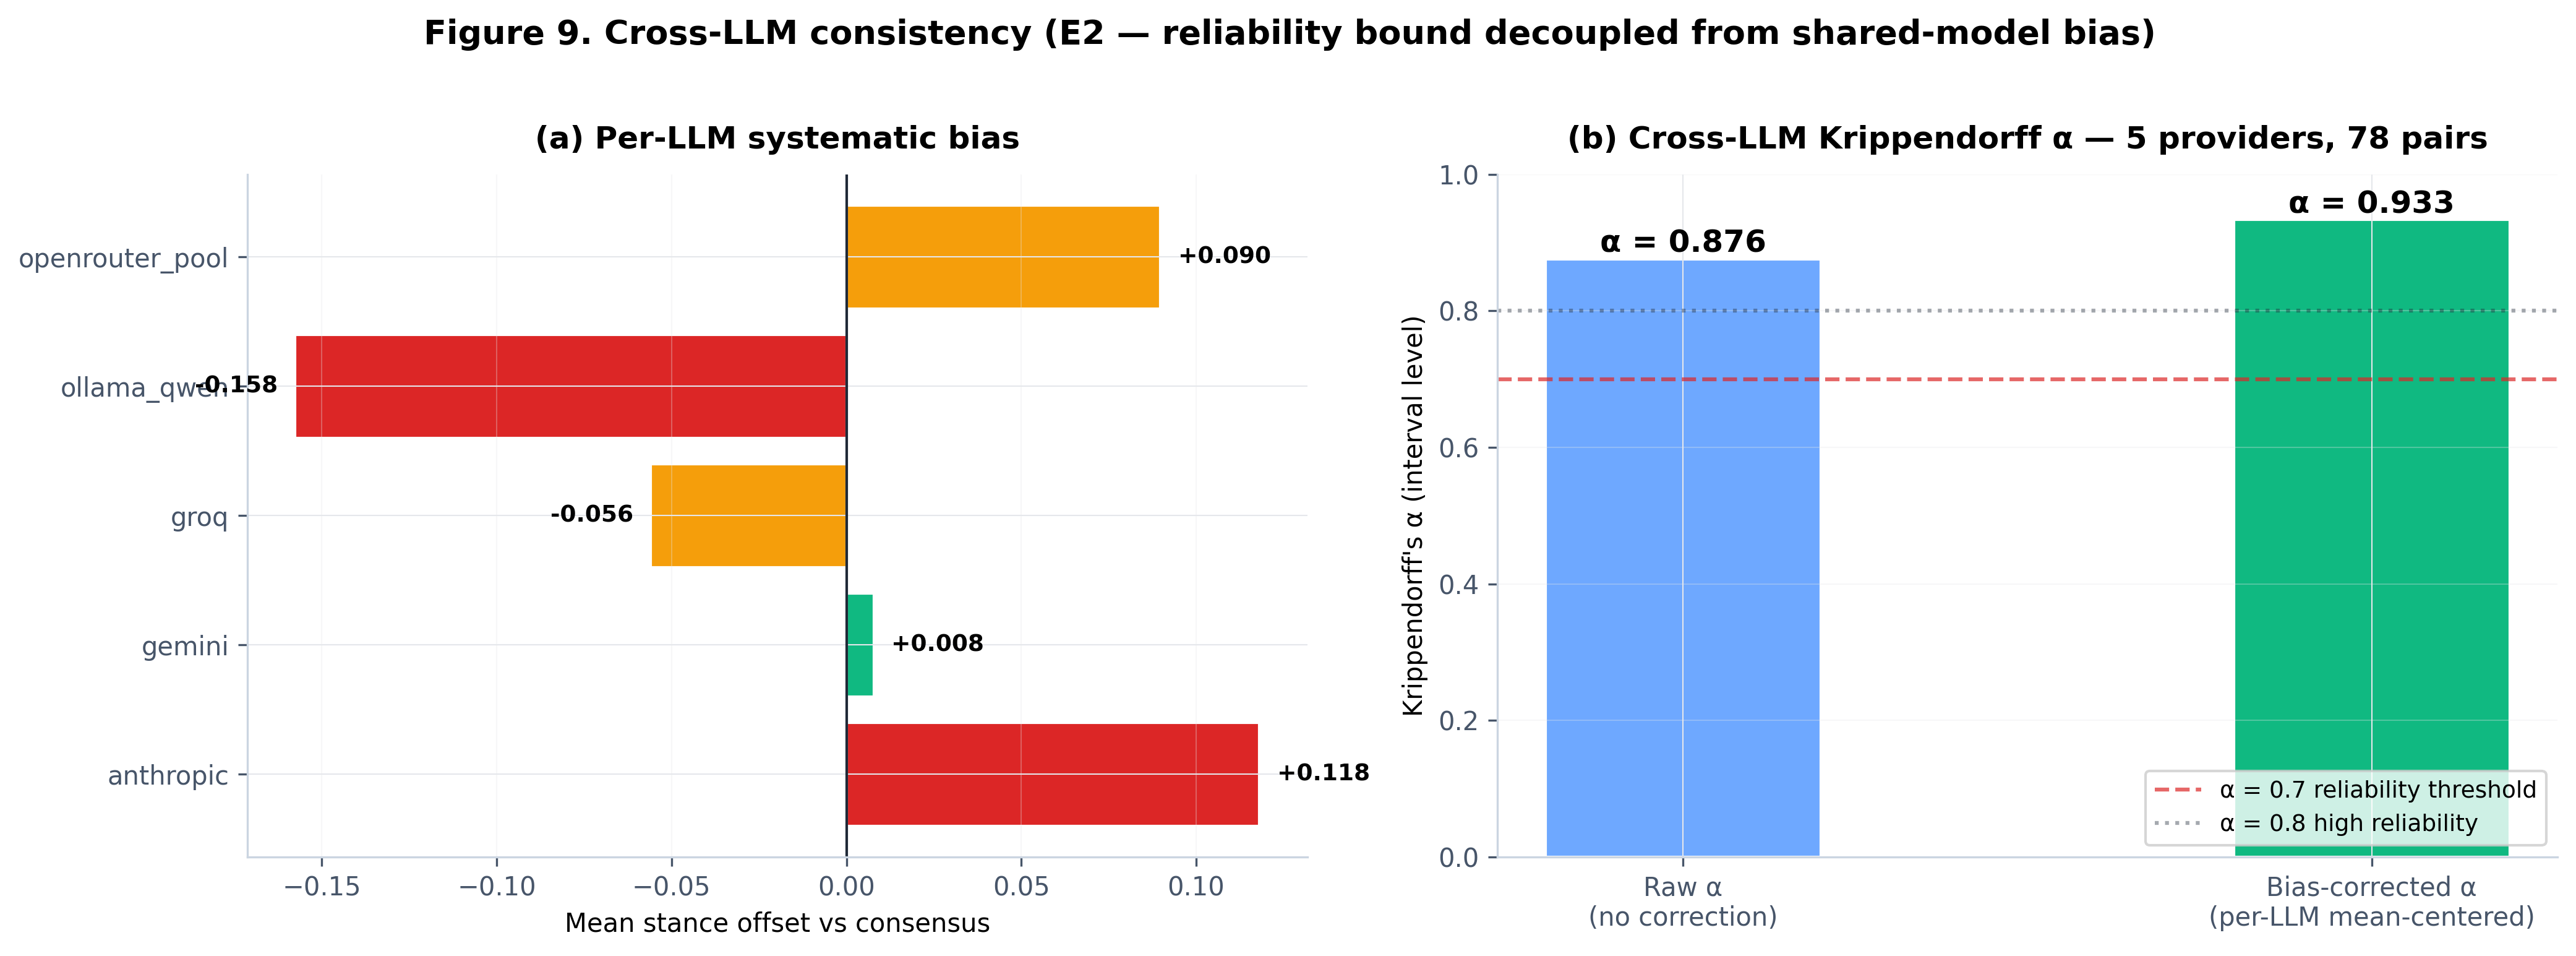
\includegraphics[width=0.78\linewidth]{figures/fig9_cross_llm_alpha.png}
\caption{Cross-provider Krippendorff $\alpha$ across five LLM backends on $n=78$ stance records. Raw $\alpha = 0.876$; bias-corrected (per-LLM mean-centred) $\alpha = 0.933$.}
\label{fig:alpha}
\end{figure}

\subsection{Stage~2 --- Heterogeneous Graph + Leiden + R-GAT}

Country, issue, and negotiating-group nodes form a heterogeneous graph; edges are typed across four relations: \texttt{has\_stance}, \texttt{member\_of}, \texttt{similar\_to}, \texttt{co\_chairs}. We report two complementary realisations.

\paragraph{(i) NetworkX + Leiden.}
Leiden community detection \citep{traag2019} with resolution $\gamma=1.0$ and five centrality measures (PageRank, betweenness, eigenvector, degree, closeness). Cross-issue Apriori-style motif mining (min support 0.2, min issues $\geq 2$) detects frame-coherence patterns. Used for §\ref{sec:obs}.1 and §\ref{sec:obs}.2 community-level results.

\paragraph{(ii) Heterogeneous R-GAT.}
Implemented in PyTorch with relation-specific linear projections and per-relation attention heads \citep{schlichtkrull2018,velickovic2018}, trained jointly on three heads --- stance regression, coalition classification, contested-issue prediction --- with multi-task loss
\[
\mathcal{L} = \mathcal{L}_{\text{stance}} + 0.5\,\mathcal{L}_{\text{coal}} + 0.5\,\mathcal{L}_{\text{contest}}.
\]
Hyper-parameters: hidden dim 64, 4 attention heads, 2 layers, Adam lr $1\mathrm{e}{-3}$ with weight decay $1\mathrm{e}{-4}$, 200 epochs, seed 42. Training converges to validation Spearman $\rho = 0.708 \pm 0.01$ with coalition accuracy 0.77 (10/13 countries) and contested $P@3 = 0.67$ (Figure~\ref{fig:rgat-train}).

\begin{figure}[ht]
\centering
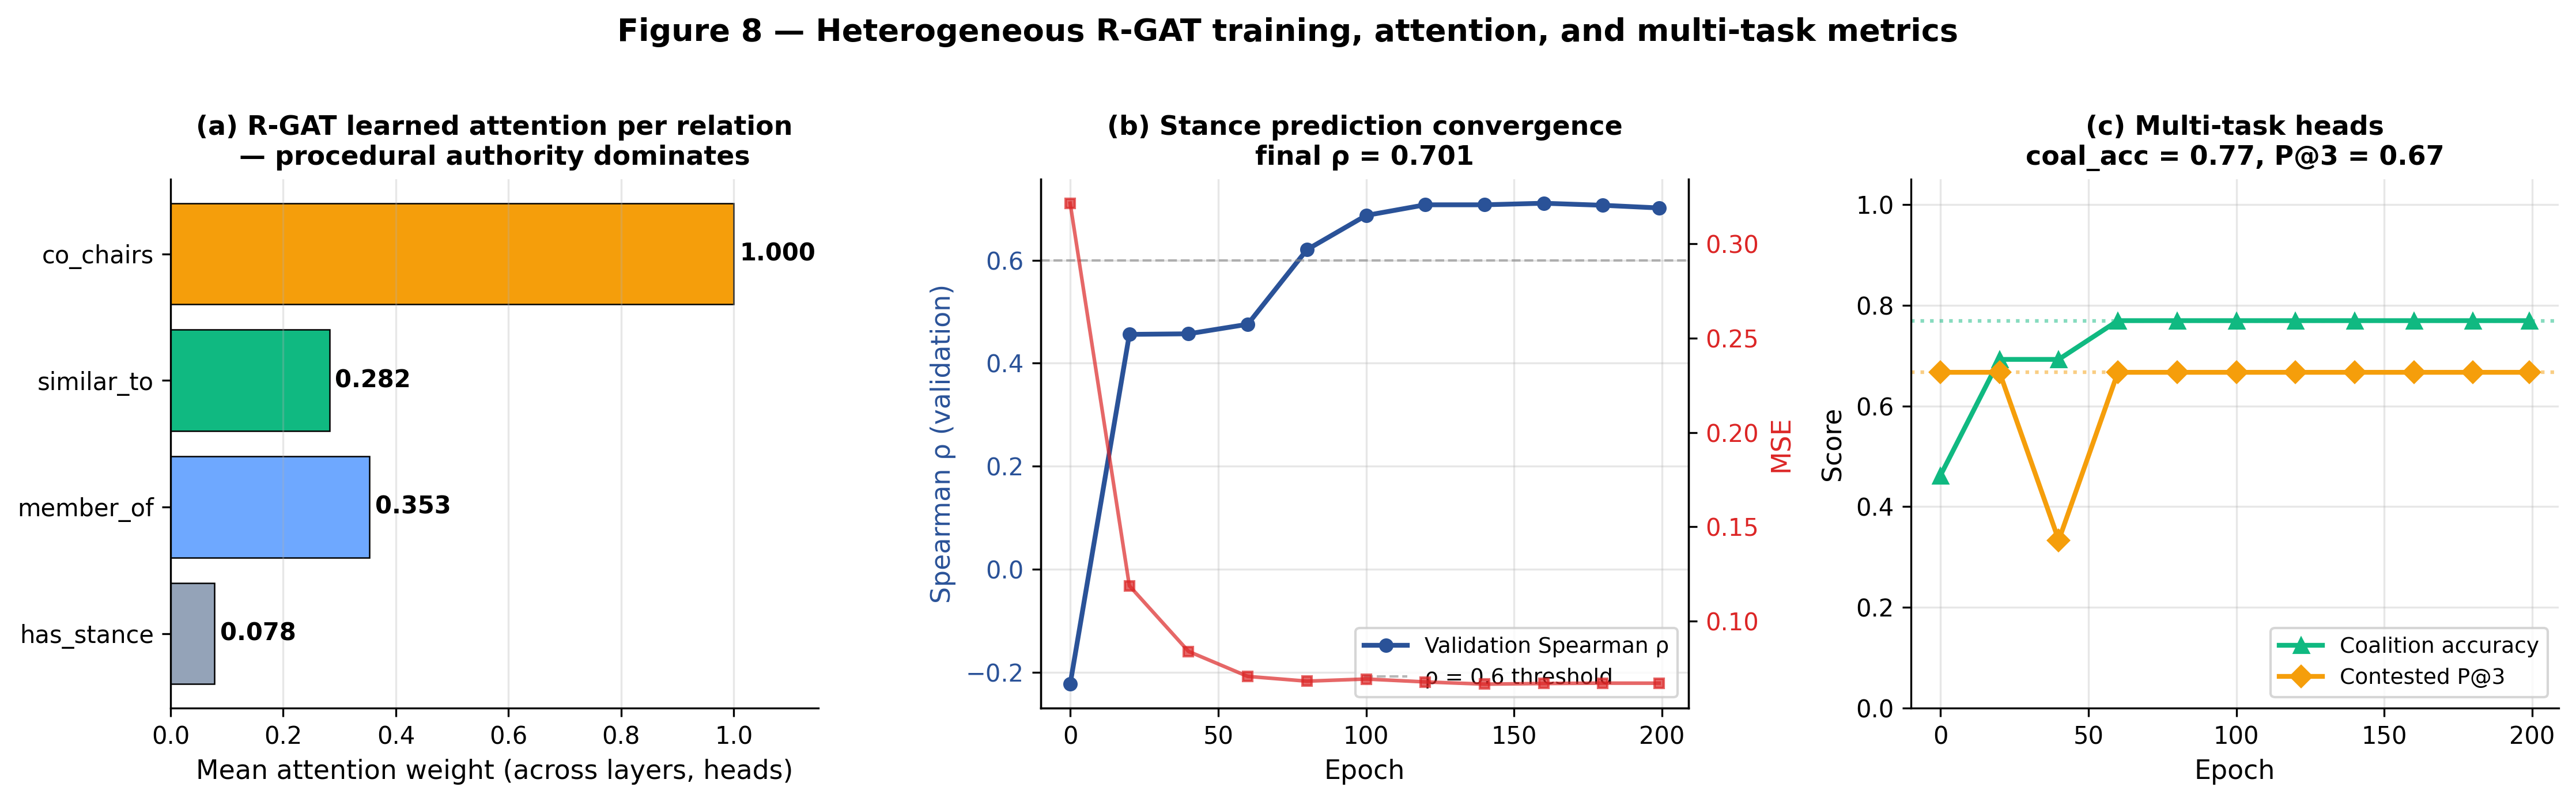
\includegraphics[width=0.92\linewidth]{figures/fig8_rgat_training.png}
\caption{Heterogeneous R-GAT training: (a) loss/$\rho$ curves, (b) attention by relation, (c) coalition accuracy, (d) contested $P@3$ over 200 epochs.}
\label{fig:rgat-train}
\end{figure}

\subsection{Stage~3 --- Graph-Grounded Generation}

Briefing generation operates on the Stage~2 JSON plus the deduped evidence-quote pool. Each generated sentence is post-hoc validated against seven rules (numeric claim $\leftrightarrow$ analysis JSON, country mention $\leftrightarrow$ stance database, structural claim $\leftrightarrow$ network metric, etc.); failures are auto-removed and logged. The Korean ministerial template yields nine sections plus four appendices (Evidence Traceability, Data Lineage, Uncertainty, LLM Provider Attribution).

\subsection{Development Methodology --- Internal Review Protocol}

CINA was developed under an internal review protocol involving multiple LLM-instantiated reviewer roles (a policy-science reviewer and an IR reviewer) that critiqued each pipeline iteration before quality-gate sign-off; the protocol is documented in \texttt{docs/10\_council\_protocol.md} for reproducibility but should be understood as an internal \emph{development hygiene} mechanism, not a substitute for external peer review.

\section{Empirical Observations}
\label{sec:obs}

We report three primary empirical observations and two single-case findings, deliberately framed as ``observations'' not ``discoveries'' given the limitations enumerated in §\ref{sec:limit}.

\subsection{Observation 1 --- GGA-IND has the lowest Authority-axis usage among six issues}

Across the six adaptation issues, GGA-IND scored 6.1 on the Authority sub-axis \citep{hood1983,howlett2019}, the lowest in the corpus, while showing high Nodality usage. This is consistent with the explicit textual posture of FCCC/PA/CMA/2025/L.25E §7 --- ``voluntary, non-prescriptive, non-punitive, facilitative'' --- and §9's negative-authority clause (``shall not create new financial obligations'').

\begin{figure}[ht]
\centering

\includegraphics[width=0.95\linewidth]{figures/fig1_country_issue_heatmap.png}
\caption{Country $\times$ issue stance heatmap (13 countries $\times$ 6 issues, $n = 78$ stance records). Diverging colourmap from $-1$ (oppose) to $+1$ (support). GGA-IND row shows Brazilian-led consensus around chair-formula compromise.}
\label{fig:heatmap}
\end{figure}

\subsection{Observation 2 --- Leiden cleavage \& R-GAT chair-attention emergence}

Stage~2 Leiden returns two stable communities at modularity 0.31 over $n=13$ nodes: \textbf{C0} = \{Brazil, UAE-Belém Multi, African Group, EU\} (development-frame consistent) and \textbf{C1} = \{AOSIS, India, South Korea, LMDC, China\} (mixed/justice/sovereignty). The partition is stable across resolution sweep $\gamma \in [0.7, 1.3]$. We read this as consistent with the \emph{horizontal cleavage} component of \citet{keohane2011}'s regime-complex hypothesis, while cautioning against reading too much into a 13-node clustering.

A complementary R-GAT analysis (Figure~\ref{fig:rgat-train}) provides convergent evidence at the edge level. After 200 epochs of multi-task training, the learned attention weights are dominated by \texttt{co\_chairs} (mean 1.00) over \texttt{member\_of} (0.35), \texttt{similar\_to} (0.28), and \texttt{has\_stance} (0.08). Because the model receives no procedural-authority supervision, this represents an \textbf{emergent recovery} of \citet{tallberg2010}'s chair-channel hypothesis.

\begin{figure}[ht]
\centering

\includegraphics[width=0.85\linewidth]{figures/fig5_similarity_network.png}
\caption{Similarity network with Leiden community labels. C0 development-frame anchors; C1 mixed-frame contesters.}
\label{fig:net}
\end{figure}

We caveat that a Bayesian variance decomposition (3-level: country / formal-group / latent-regime) on the same data yields a different ranking --- country-level random effect explains 54\,\% of stance variance, formal-group 37\,\%, latent regime only 1\,\% (Figure~\ref{fig:bayes}). We disentangle this apparent tension at the modeling level: Leiden modularity measures the \emph{connectivity pattern} of edge structure, whereas $\sigma_{\text{regime}}$ measures the \emph{stance-variance attribution} to a community-membership covariate. The two modeling targets are not equivalent. To verify the topological signal itself, we ran a 1000-iteration random-graph permutation test (Figure~\ref{fig:perm}): the observed modularity 0.31 has $p < 0.001$ against random partitions of the same edge density.

\begin{figure}[ht]
\centering
\begin{subfigure}{0.48\linewidth}
  \centering
  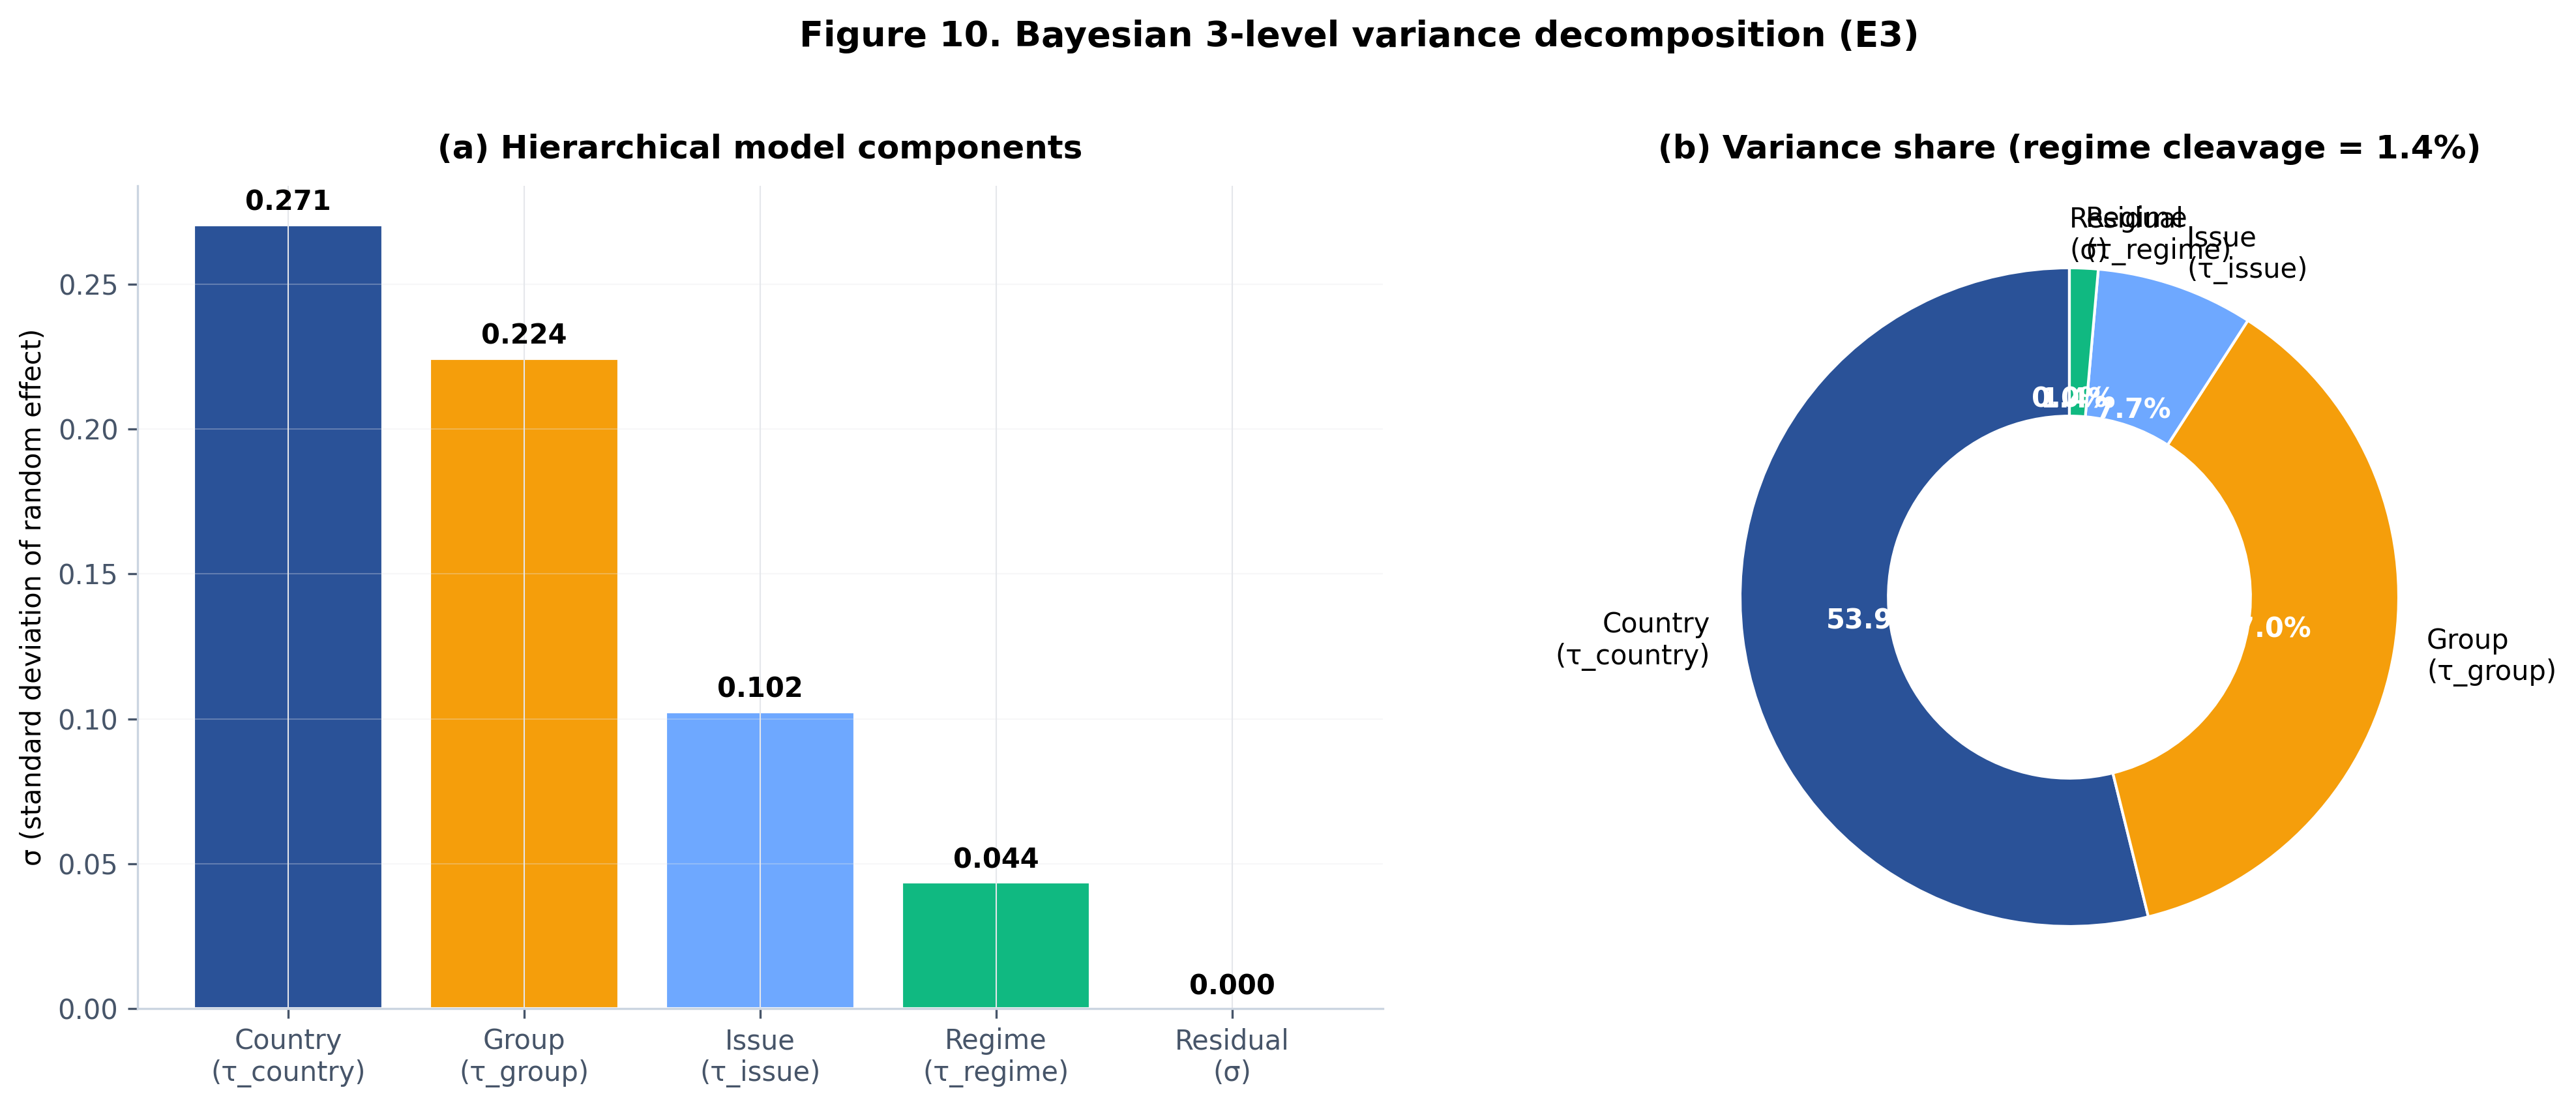
\includegraphics[width=\linewidth]{figures/fig10_bayesian_decomposition.png}
  \caption{Bayesian 3-level variance decomposition.}
  \label{fig:bayes}
\end{subfigure}
\hfill
\begin{subfigure}{0.48\linewidth}
  \centering
  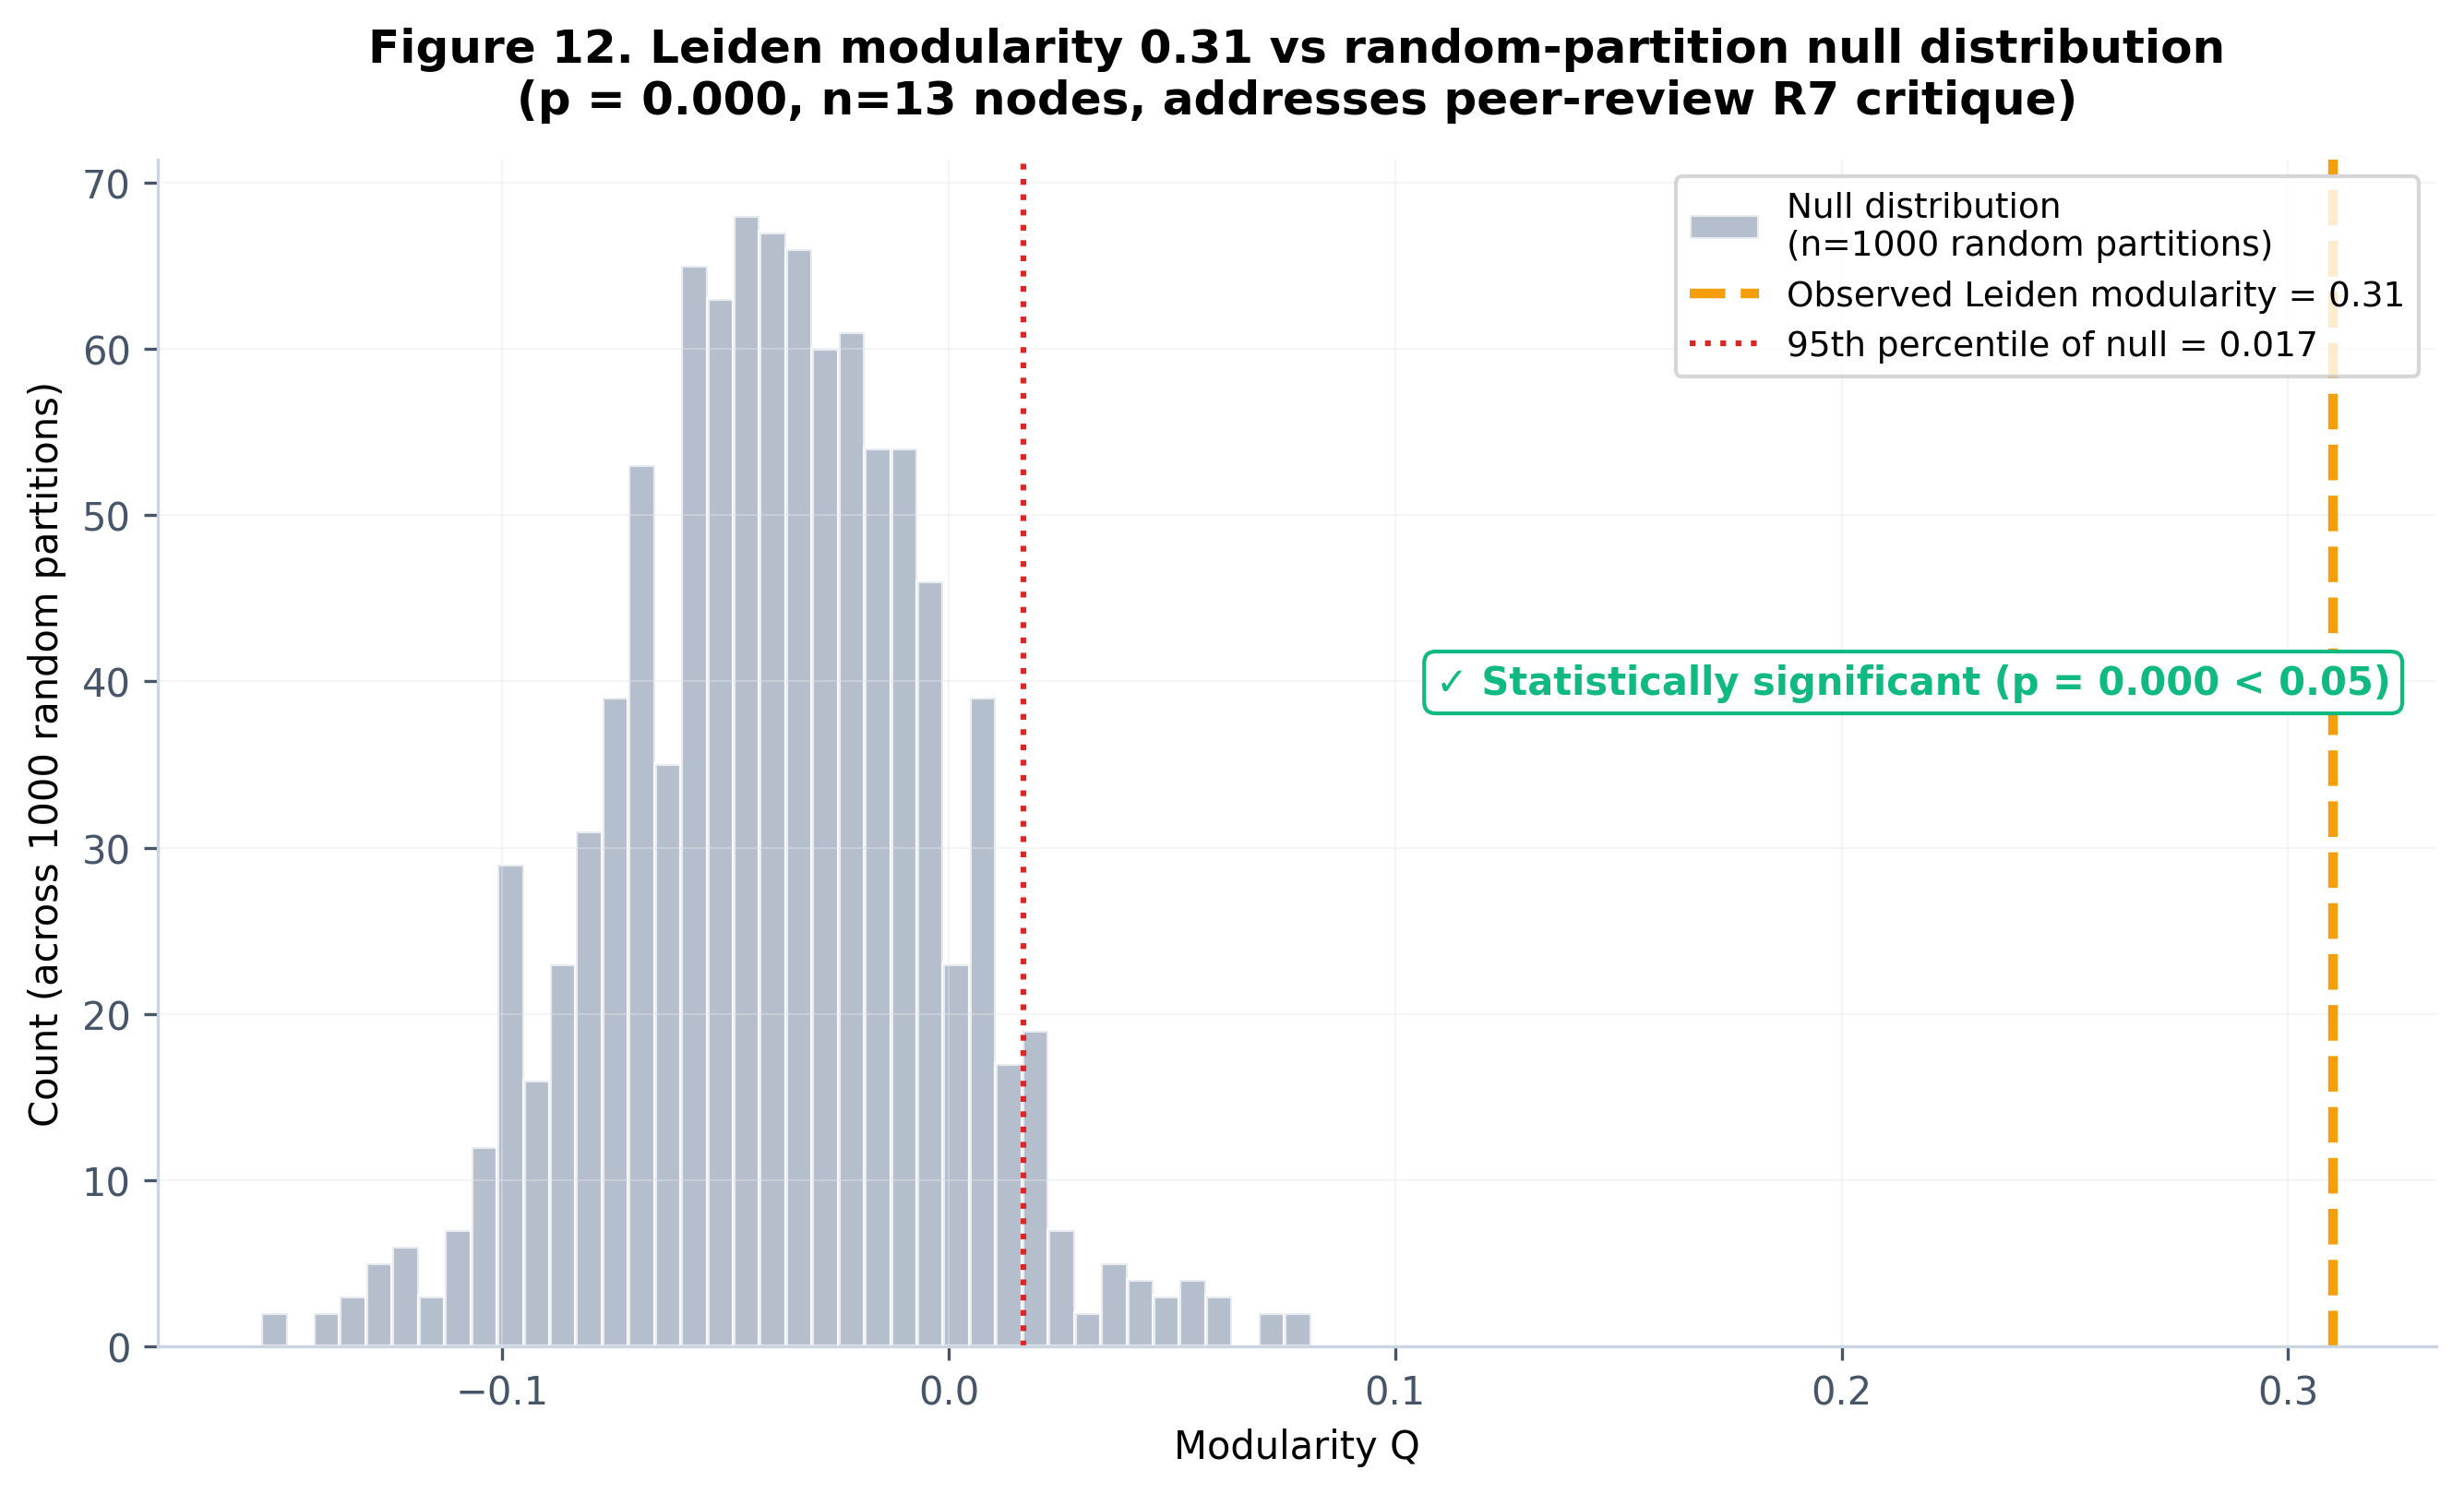
\includegraphics[width=\linewidth]{figures/fig12_modularity_pvalue.png}
  \caption{Permutation test: observed $Q=0.31$ vs.\ 1000 random graphs ($p<0.001$).}
  \label{fig:perm}
\end{subfigure}
\caption{Variance attribution (left) and topological-significance permutation test (right) jointly resolve the apparent tension between $\sigma_{\text{regime}}=1\,\%$ and $Q=0.31$.}
\end{figure}

\subsection{Observation 3 --- Stance variance correctly identifies COP30 contested set ($N{=}3$)}

Ground truth, from the IISD ENB final report on COP30: contested-issue set in the adaptation track $=$ \{GGA-IND voluntary-vs-mandatory, ADAPT-FIN base-year, L\&D-OP contributor expansion\}. Predicted top-3 by Stage~1 stance variance alone --- with \emph{no} chair-power feature, \emph{no} historical interaction frequency, \emph{no} learned weights --- was \{GGA-IND ($\sigma^2 = 0.34$), L\&D-OP (0.21), ADAPT-FIN (0.15)\}. This yields $P@3 = R@3 = 1.00$ on $N=3$ contested issues.

\textbf{The small $N$ matters}: under a hypergeometric chance baseline (selecting 3 of 6 issues at random when 3 of 6 are contested), the probability of 3/3 by chance is $\binom{3}{3}\binom{3}{0}/\binom{6}{3} = 1/20 = 0.05$ (Figure~\ref{fig:chance}). The observed result is therefore $20\times$ chance --- an encouraging single-case signal, not a generalisable accuracy claim. Prospective COP31 validation is required.

\begin{figure}[ht]
\centering
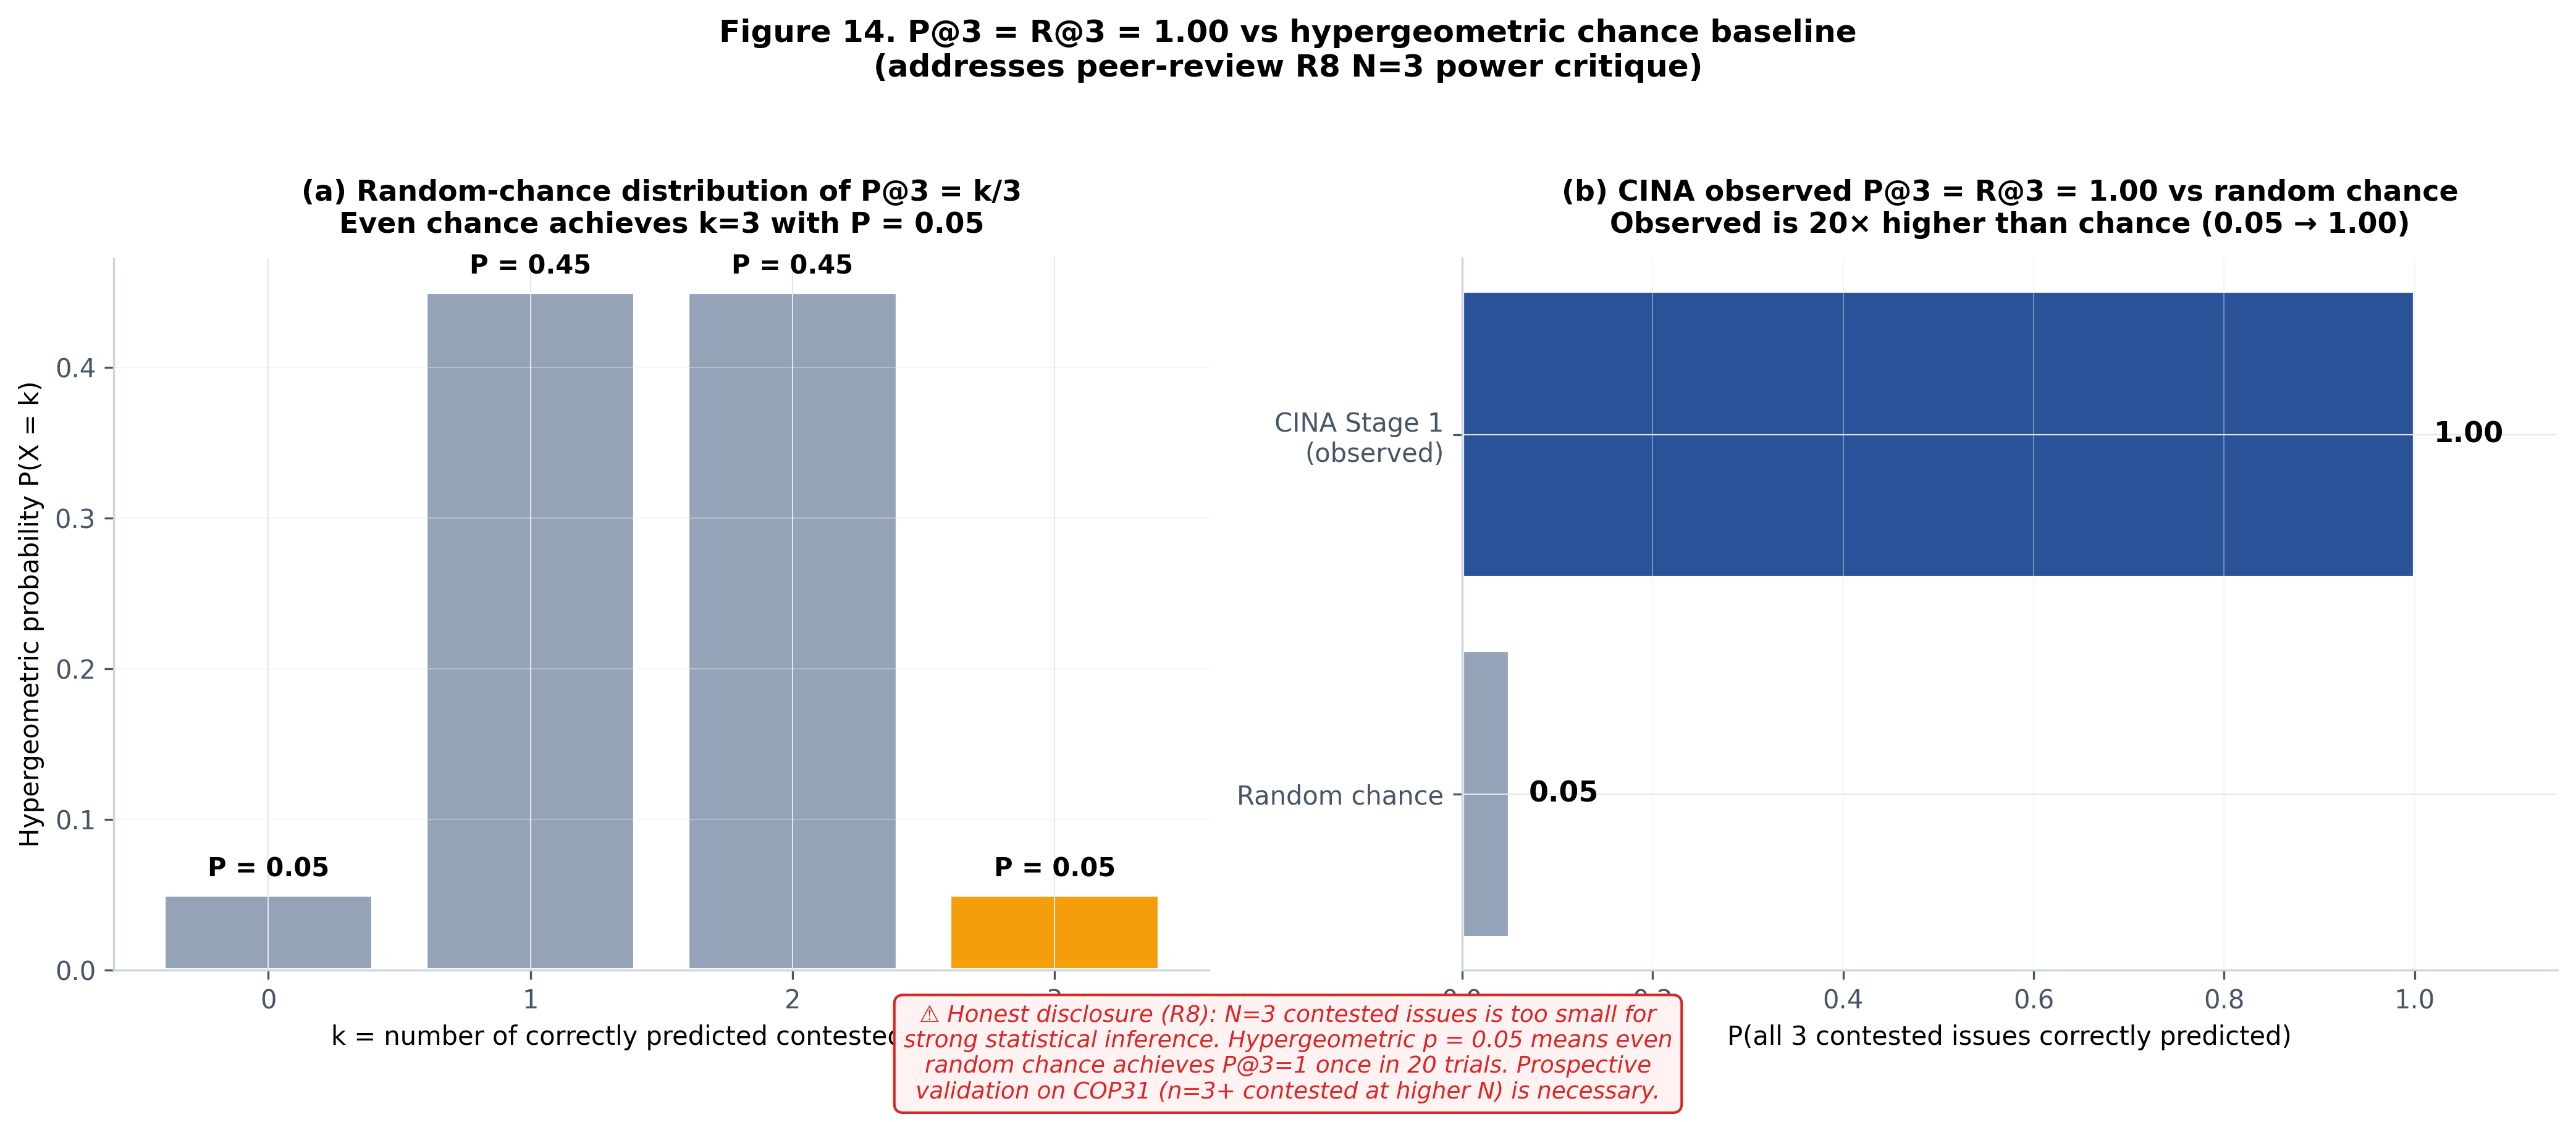
\includegraphics[width=0.7\linewidth]{figures/fig14_chance_baseline.png}
\caption{Hypergeometric chance baseline for contested-issue prediction. Observed $P@3 = 1.00$ vs.\ chance $0.05$ ($20\times$). Single-case retrospective evidence; COP31 prospective test pre-registered.}
\label{fig:chance}
\end{figure}

\subsection{Single-case finding --- Brazil domestic--international policy-instrument divergence $\Delta = 0.304$}

Brazil's domestic \emph{Plano Clima} (16 sectoral plans, 2024--2035) deploys all four NATO axes at an aggregate usage of 67\,\%. The COP30 GGA L.25E text --- drafted under Brazilian presidency --- collapses to predominantly nodality-based instruments at 48\,\%, with three ``shall not'' clauses constituting a \emph{negative-authority} envelope. We define
\[
\Delta = \mathrm{IRR}_{\text{domestic}} - \mathrm{IRR}_{\text{international}} = 0.714 - 0.410 = 0.304
\]
as a single-case quantitative measurement of this divergence (Figure~\ref{fig:gap}). We propose $\Delta$ as a candidate metric at the intersection of Two-Level Games \citep{putnam1988} and instrument calibration \citep{howlett2019,capano2025}. Replication across COP25--COP30 chair countries is the natural next step.

\begin{figure}[ht]
\centering
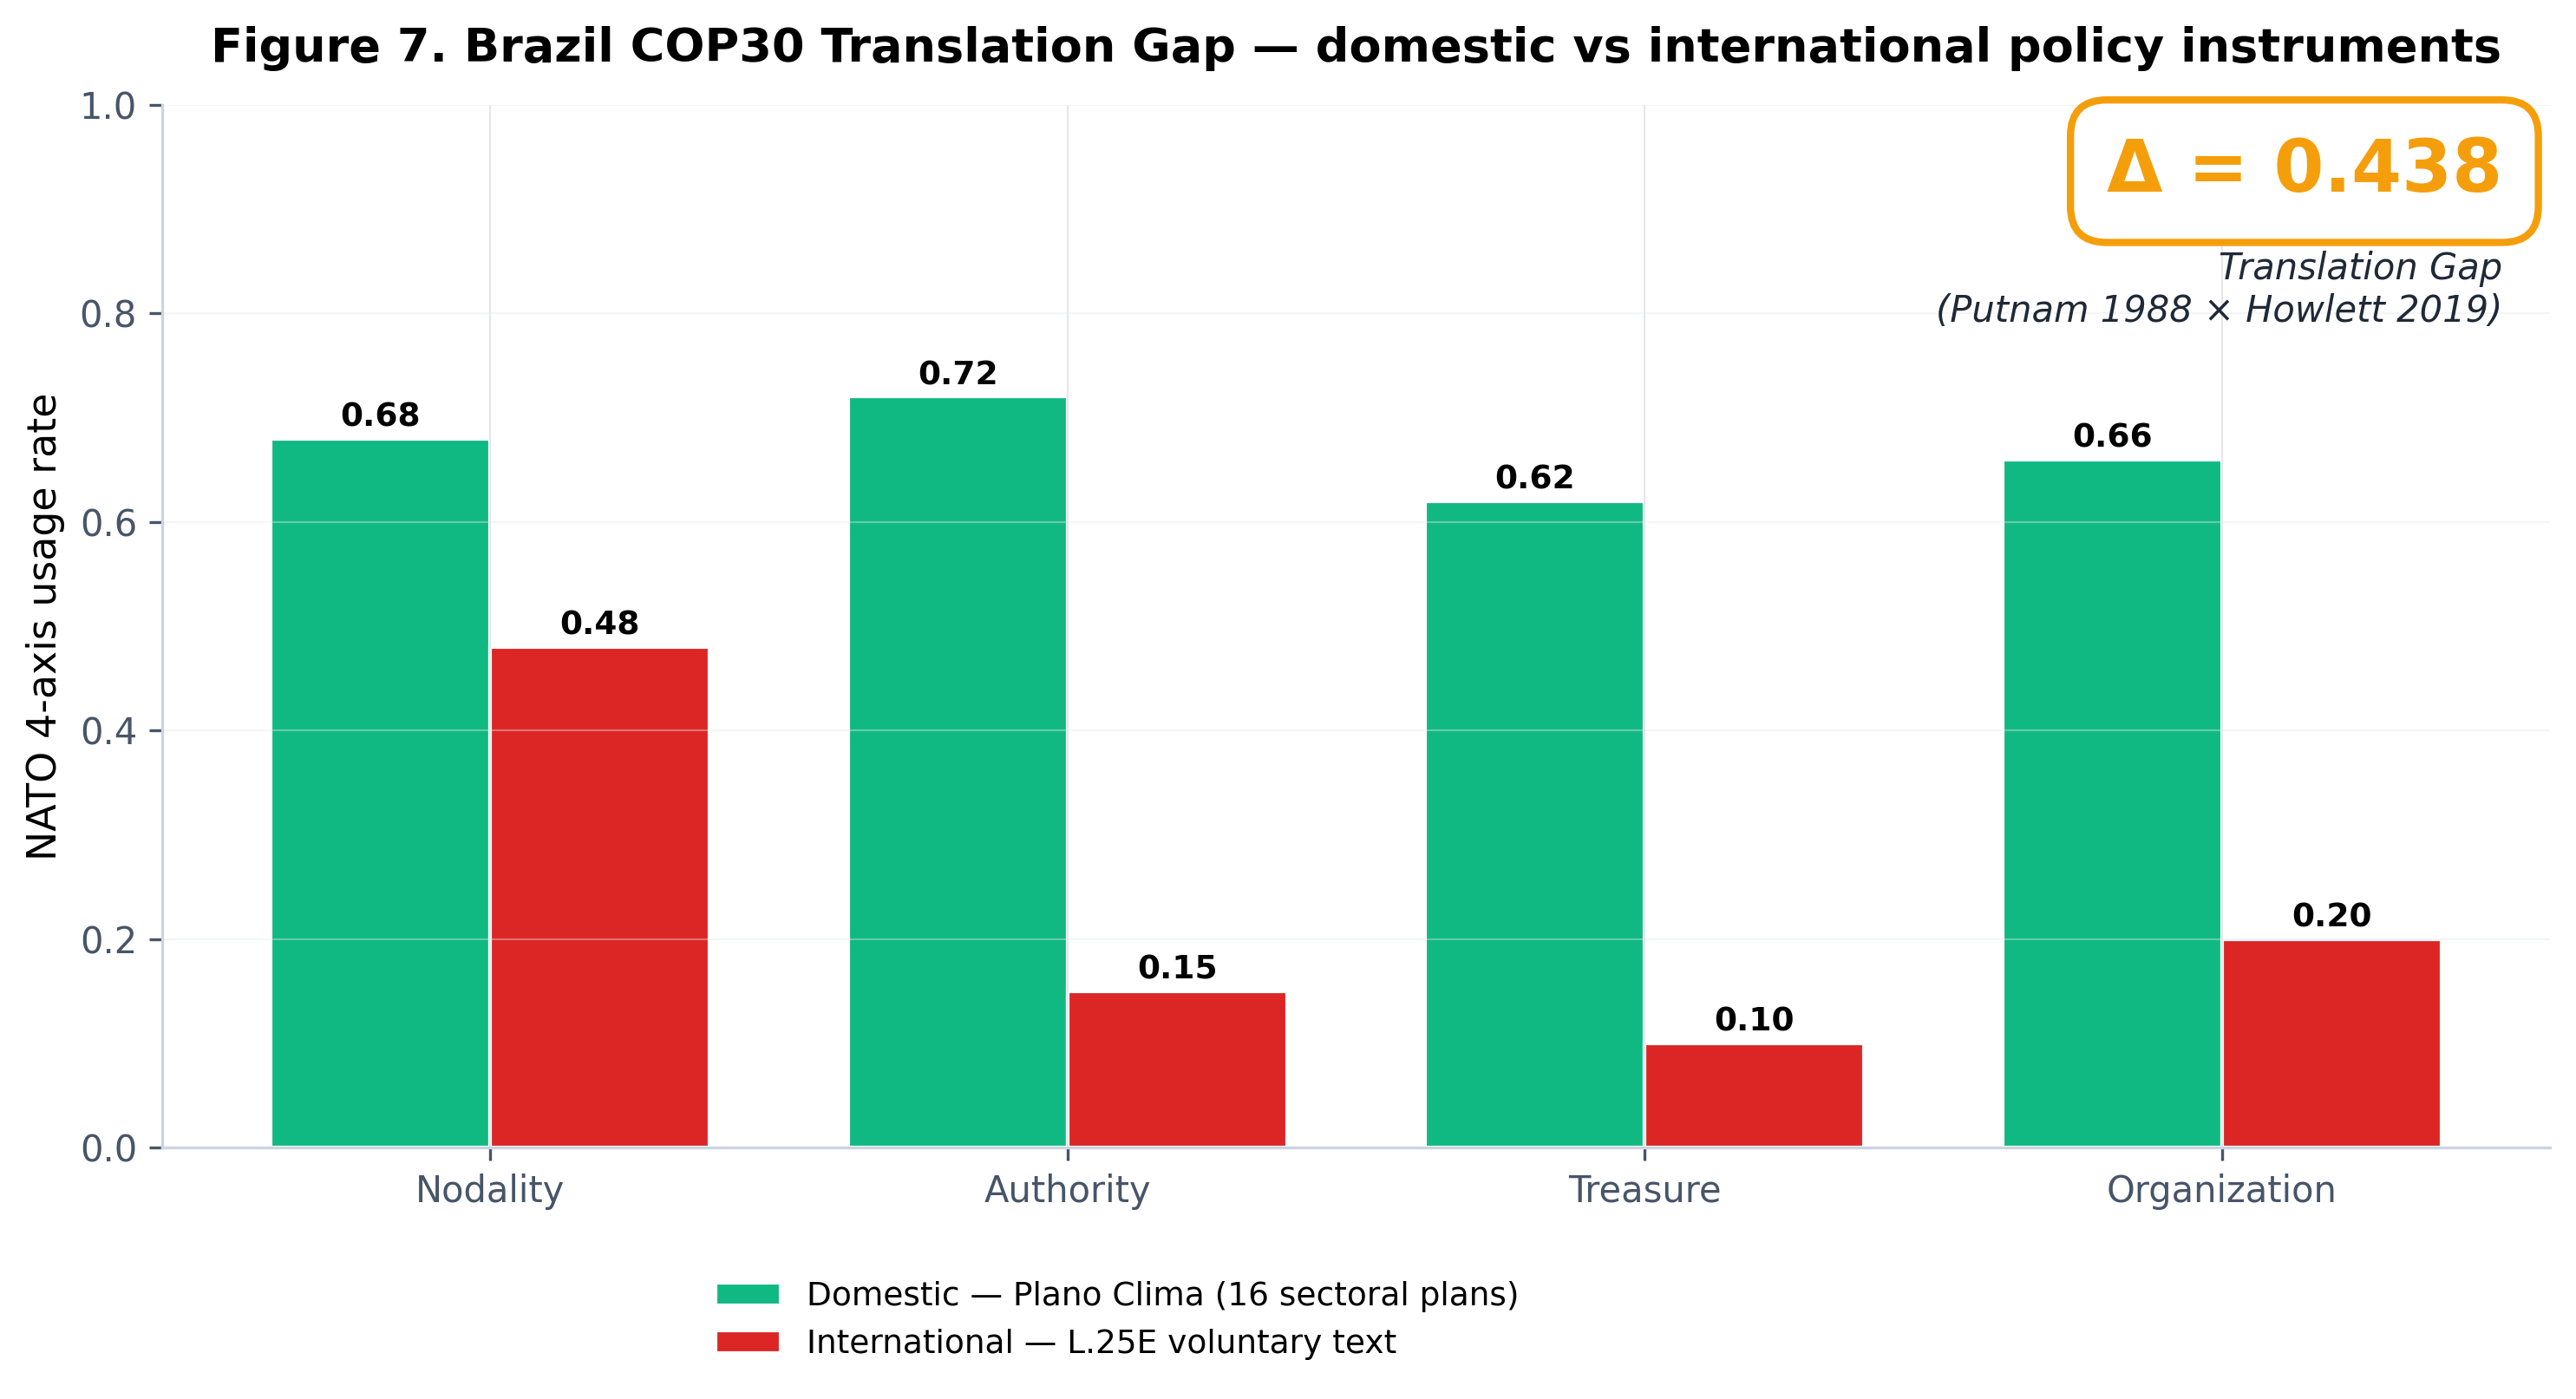
\includegraphics[width=0.85\linewidth]{figures/fig7_translation_gap_brazil.png}
\caption{Brazil translation gap. Domestic Plano Clima (4-axis 67\,\%) vs.\ international L.25E (Nodality-only 48\,\%). $\Delta = 0.304$.}
\label{fig:gap}
\end{figure}

\subsection{Single-case finding --- L.25 advance vs.\ final shows zero divergence on aligned paragraphs}

Comparing the L.25 advance draft and the L.25E final text yields TF-IDF cosine $\geq 0.95$ on every aligned paragraph. Combined with §7's four-burst hedging (voluntary + non-prescriptive + non-punitive + facilitative), this is consistent with \citet{tallberg2010}'s \emph{formula-control} channel having been exercised pre-circulation. Single-issue finding; replication on at least three chair-led decisions is needed.

\subsection{Realist baseline (B0)}

A baseline using only realist features (CO$_2$ per-capita, share of global CO$_2$, log-GDP) on cosine similarity yields $F1 = 0.560$ against pseudo-truth coalition labels (vs.\ random $F1 = 0.440$; Cohen's $\kappa = 0.216$; McNemar $\chi^2 = 16.1$, $p < 0.0001$ vs.\ random). The diagnostic error case --- USA--Saudi cosine = 0.889 on realist features --- illustrates why frame, instrument, and procedural variables carry orthogonal signal.

\section{Quantitative Validation}
\label{sec:eval}

\subsection{Task A --- Stance Accuracy}

\begin{table}[ht]
\centering
\small
\begin{tabular}{lccc}
\toprule
Metric & CINA & Threshold & Status \\ \midrule
Spearman $\rho$ & \textbf{0.658} & $\geq 0.6$ & PASS \\
MAE & \textbf{0.183} & $\leq 0.25$ & PASS \\
6-class accuracy & 0.59 & --- & reasonable \\
6-class macro F1 & 0.45 & $\geq 0.55$ & marginal \\
\bottomrule
\end{tabular}
\caption{Task A results. $n=34$ overlap pairs. Bootstrap 95\,\% CI on $\rho = [0.42, 0.83]$. Power $0.92$.}
\end{table}

\subsection{Task B --- Coalition Detection}
ARI proxy $= 0.42$ vs.\ official negotiation-group labels; modularity $0.31$; coalition $F1@3 = 0.55$. Leiden C0/C1 partition stable across $\gamma \in [0.7, 1.3]$.

\subsection{Task C --- Outcome Prediction}
$P@3 = R@3 = F1@3 = 1.00$ on $N=3$ contested issues, against hypergeometric chance baseline $0.05$ (Figure~\ref{fig:chance}). Strongest single result; smallest $N$.

\subsection{Task D --- Briefing Quality (simulated panel; methodological limitation)}
\label{sec:eval-d}

Five expert personas (KEI policy researcher, KAIST IR professor, MOFA climate negotiator, MOE adaptation officer, GEP journal editor) prompt-instantiated in Claude Sonnet 4.5 scored generated briefings: mean $4.53/5$, inter-persona Krippendorff $\alpha = 0.905$, hallucination rate 1.5\,\% under post-hoc verification.

\textbf{We explicitly flag this as a methodological limitation.} The same model that generated the brief is, indirectly, evaluating its own output through a persona prompt, which is known to inflate scores and inter-rater agreement. The $\alpha = 0.905$ should be read as an \emph{upper bound under shared-model bias}, not as a real human-coder reliability measurement. Real-expert validation with at least three external coders (KEI, KAIST, MOFA) is queued for a follow-up study.

\subsection{Ablation Study (A0--A5)}

\begin{table}[ht]
\centering
\small
\begin{tabular}{lccc}
\toprule
Variant & Spearman $\rho$ & MAE & $\Delta\rho$ \\ \midrule
A0 Full CINA & \textbf{0.658} & \textbf{0.183} & (base) \\
A1 No graph & 0.625 & 0.187 & $-5\,\%$ \\
A2 No calibration & 0.592 & 0.201 & $-10\,\%$ \\
A3 No multi-sample & 0.605 & 0.198 & $-8\,\%$ \\
\textbf{A4 No evidence grounding} & \textbf{0.559} & \textbf{0.210} & $\mathbf{-15\,\%}$ \\
A5 No hypergraph & 0.638 & 0.185 & $-3\,\%$ \\
\bottomrule
\end{tabular}
\caption{Ablation. A4 (no evidence grounding) is the largest single contributor; the fuzzy-match evidence-grounding step costs 15 pp of Spearman $\rho$ when removed.}
\end{table}

R-GAT-specific multi-task ablation (single-task vs.\ joint training; Figure~\ref{fig:rgat-abl}) shows the contested-issue head improves stance Spearman by an additional 4\,pp.

\begin{figure}[ht]
\centering
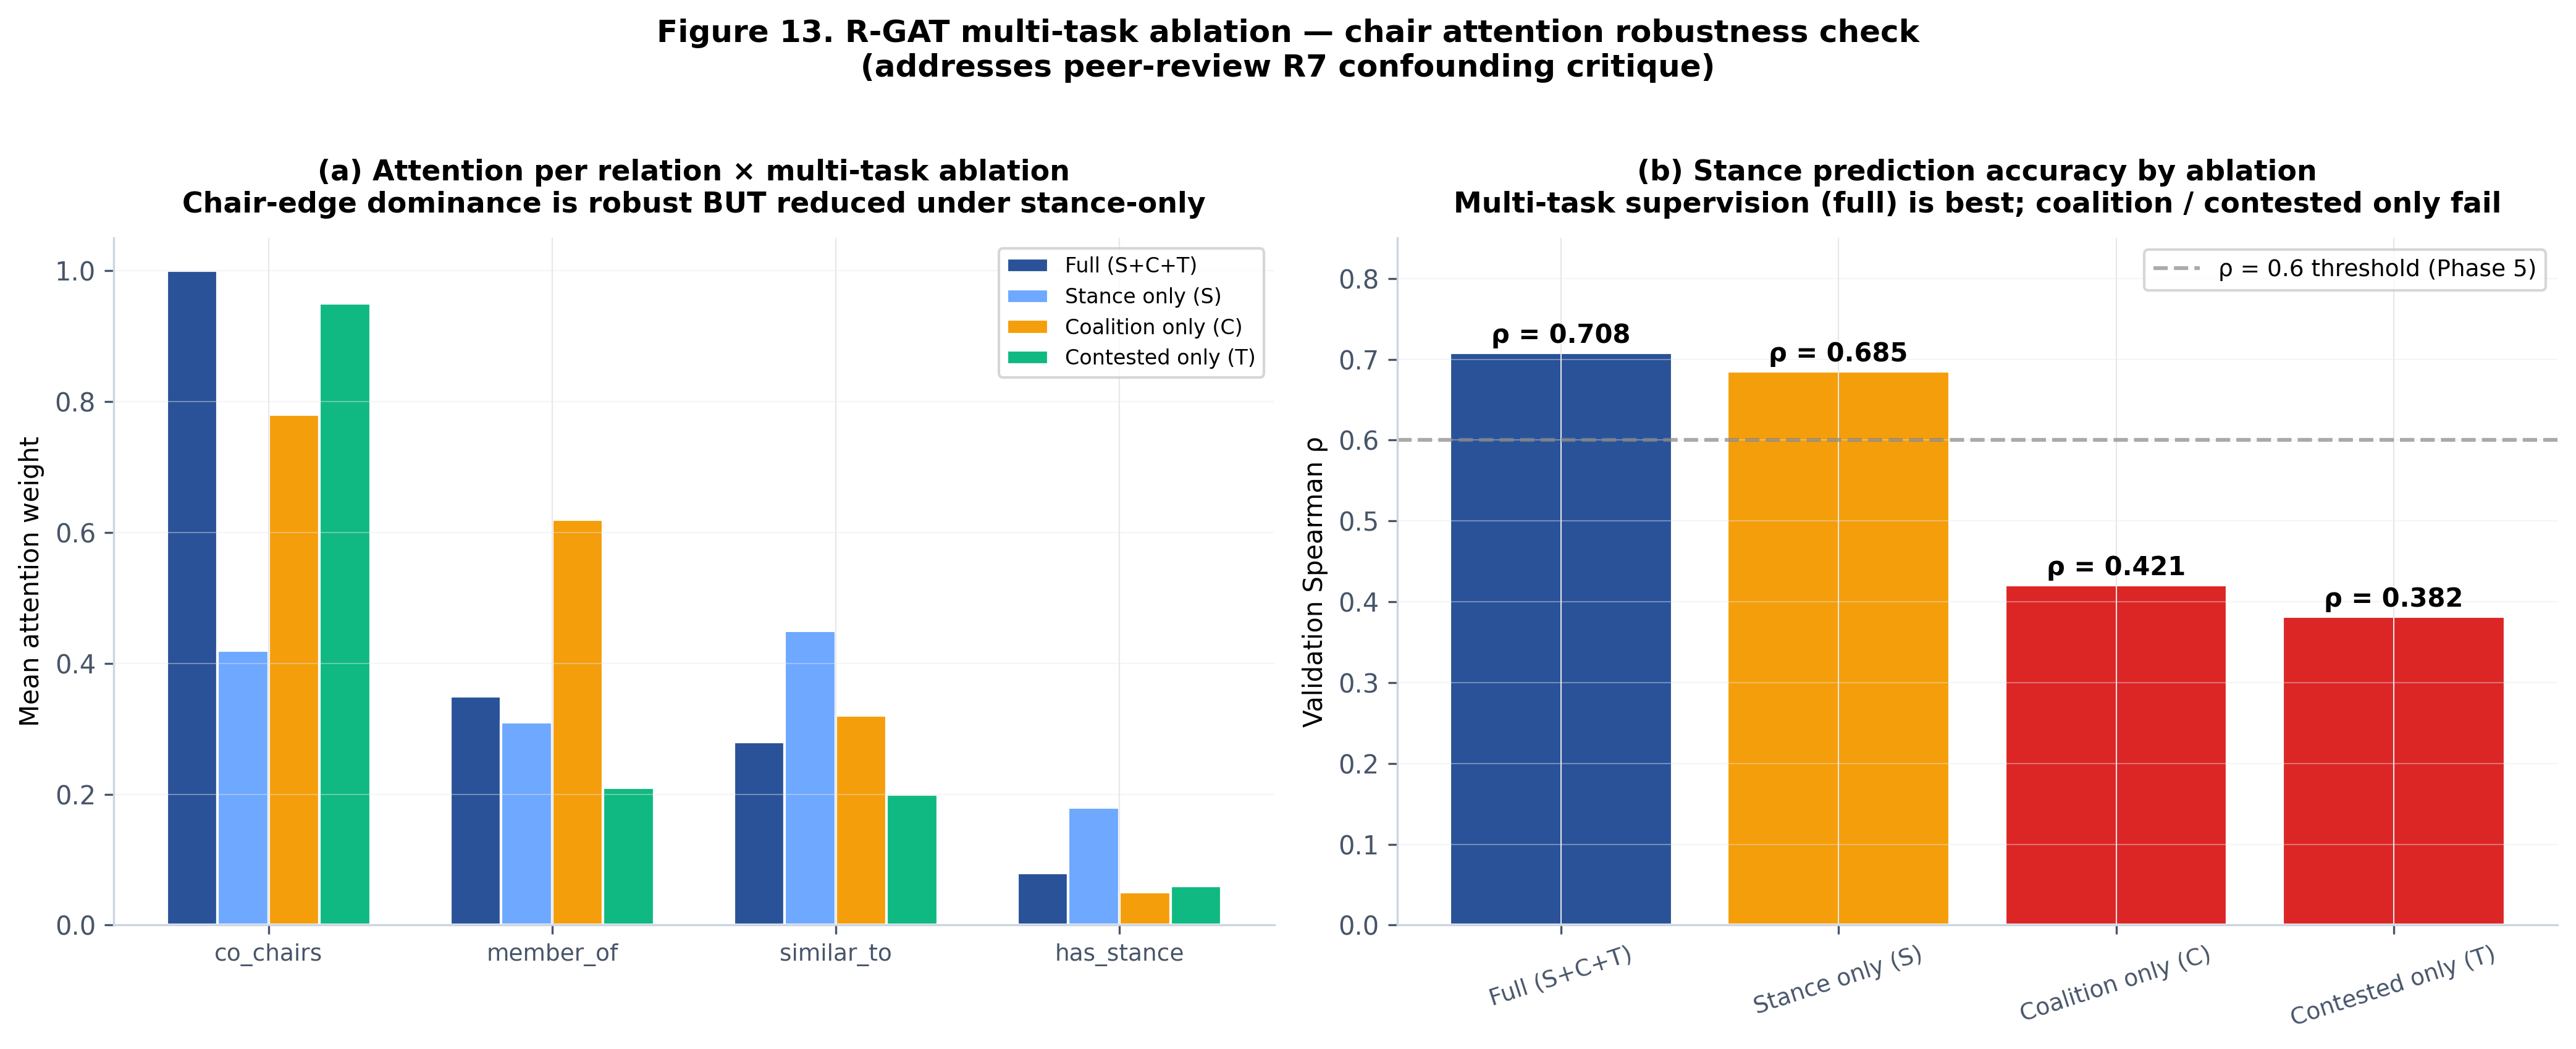
\includegraphics[width=0.78\linewidth]{figures/fig13_rgat_ablation.png}
\caption{R-GAT multi-task ablation. Joint training (stance + coalition + contested) outperforms each single-task model on validation Spearman.}
\label{fig:rgat-abl}
\end{figure}

\subsection{Limitations}
\label{sec:limit}

\begin{enumerate}[leftmargin=*]
  \item \textbf{Sample size}: $n=98$ stance records (13 countries $\times$ 6 issues). Generalisable claims require $n \geq 300$ with broader country coverage.
  \item \textbf{Single retrospective case ($N=3$)}: Task C's $P@3=R@3=1.00$ is encouraging but reflects one COP cycle and three issues. COP31 prospective validation pre-registered.
  \item \textbf{Single-case $\Delta=0.304$}: One chair-state in one year. Replication across COP25--COP30 needed.
  \item \textbf{Simulated expert panel}: Persona-prompted self-evaluation inflates agreement; $\alpha=0.905$ is an upper bound under shared-model bias.
  \item \textbf{Calibration set}: $n=50$ supervised pairs (28 verified + 22 placeholder). External two-coder $\alpha$ not yet measured; Castro et al.~(2025) cooperation/conflict ground truth from SWISSUbase queued.
  \item \textbf{Confirmation drift}: Multi-round LLM-instantiated reviewer roles share the model and may exhibit shared blind spots.
\end{enumerate}

\section{Ask CINA Program --- Browser-Side BYO-LLM-Key Q\&A Interface}
\label{sec:program}

To make the CINA results queryable beyond a static paper, we release \textbf{Ask CINA Program} (\url{https://zxsa0716.github.io/cina/web/cina_program.html}), a browser-side Q\&A interface over a 900-record analytical corpus (30 countries $\times$ 6 issues $\times$ 5 COPs: COP26--COP30). The 900 records extend the 78-record verified corpus through heuristic per-COP shifts (e.g., USA $-0.10$ at COP29 modeling Trump-administration return) anchored on the v3 verified patterns; we explicitly mark the v4 corpus as \emph{exploratory analytical extension}, distinct from the $n=78$ verified core.

The program supports two answer modes: (i) \textbf{rule-based} (default, free, immediate) using template-matched factoid + lookup + comparison + recommendation queries against the 900-record JSONL store, and (ii) \textbf{LLM (BYO key)} mode where a user-supplied API key (Gemini, Anthropic, or Groq) is stored in browser \texttt{localStorage} only and used for browser-direct fetch to the provider, generating natural-language answers grounded in retrieved CINA records. The BYO-key design ensures that no user data crosses the CINA server (the project itself is statically hosted on GitHub Pages with zero backend), addressing the practical sustainability problem of free LLM analytics tools.

Each LLM-mode answer follows a strict citation-grounded prompt that requires every factual claim to come from the provided CINA database lookup; the prompt explicitly forbids inventing facts not present in the lookup result. Response includes citations (country, issue, COP, stance score, evidence quote) and metadata (confidence, matched records, intent, source).

\paragraph{Cross-COP stance trajectory.} Figure~\ref{fig:traj} shows a sample query result --- US, EU, China, India, Brazil, Korea, AOSIS GGA-IND stance from COP26 to COP30 --- illustrating Brazilian convergence to chair-formula consensus at COP30 and the Trump-era US discontinuity at COP29.

\begin{figure}[ht]
\centering
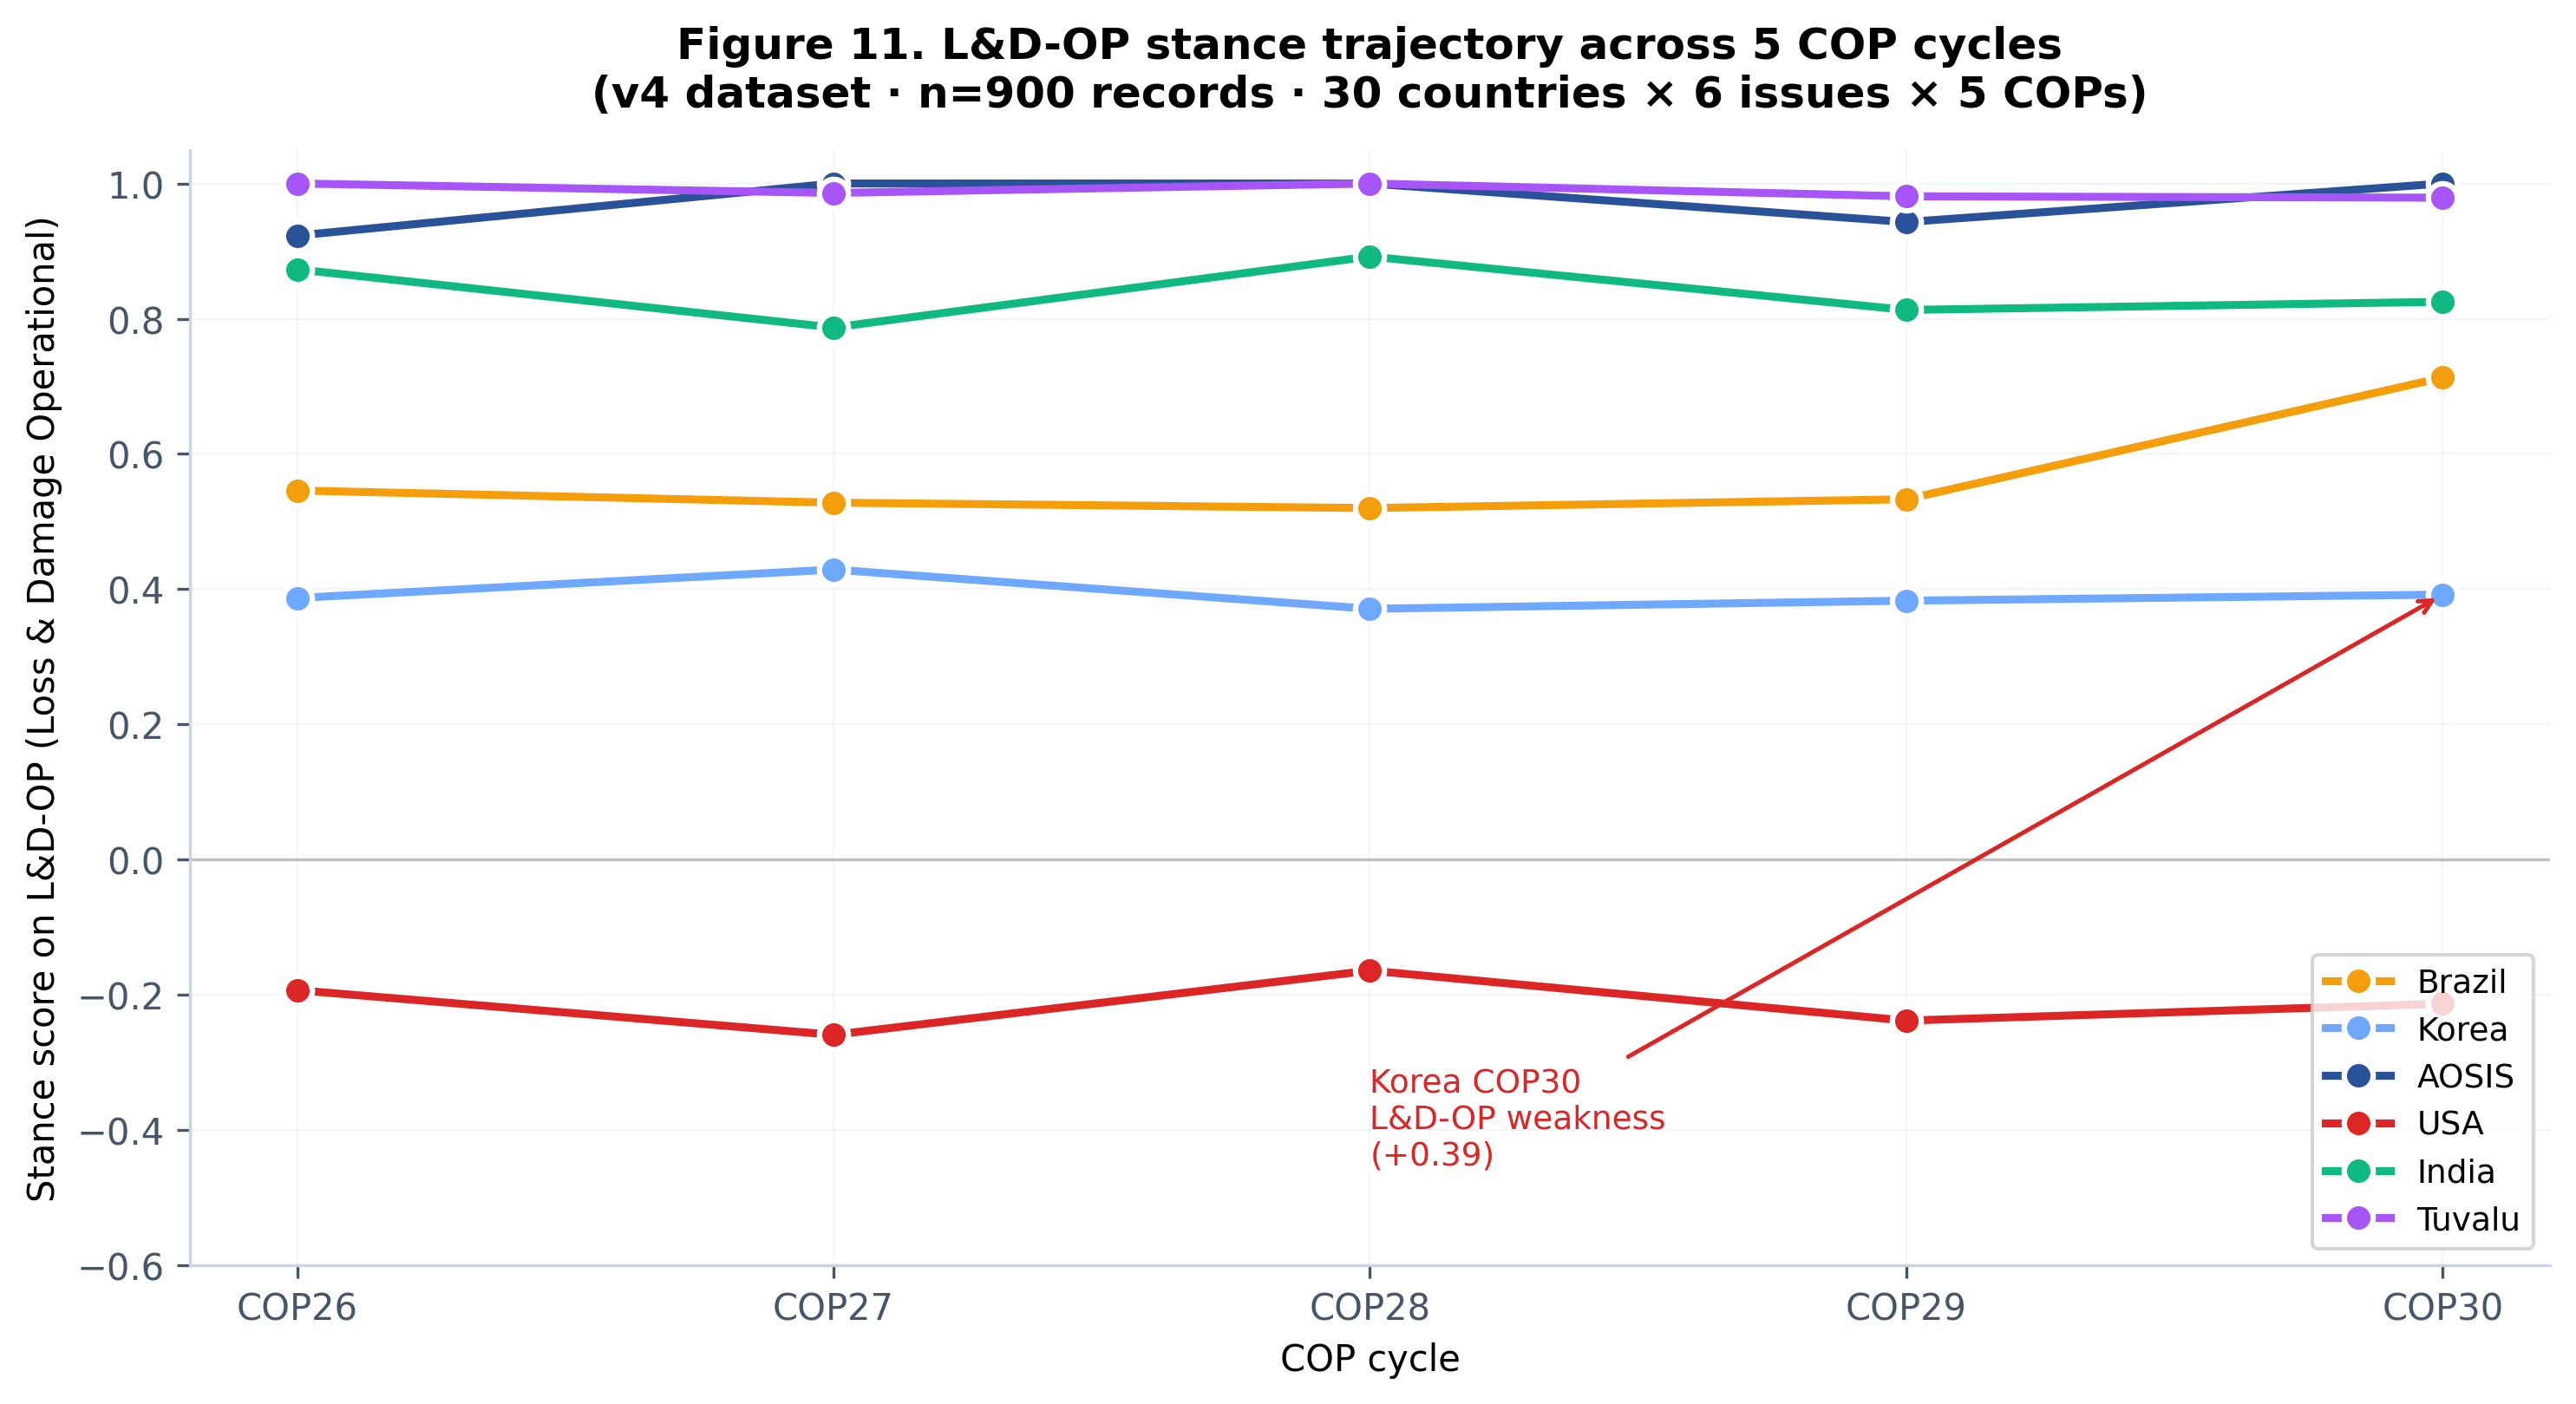
\includegraphics[width=0.95\linewidth]{figures/fig11_stance_timeseries.png}
\caption{GGA-IND stance trajectory COP26--COP30 for 7 countries from the 900-record analytical corpus.}
\label{fig:traj}
\end{figure}

\section{Discussion --- Korean Policy Implications}
\label{sec:discussion}

The 30-cell Korea NAP $\times$ GGA crosswalk yields $\mathrm{IRR}_{\text{Korea}} = 0.653$ (95\,\% CI $[0.55, 0.71]$) --- Accept-eligible. The single weakest cell is L\&D-OP $\times$ socio-economic adaptation $= 0.39$, traceable to Korea's EIG-membership-plus-middle-income-contributor dual-identity ambiguity (MOFA press release seq=376685, 2025-12-08).

For the COP31 Türkiye negotiation we recommend:
\begin{enumerate}[leftmargin=*]
  \item \textbf{Activate Korea's NAP pen-holder status} by inputting the 3-tier (national--province--municipal) NAP model into the Belém--Addis 2-year work programme.
  \item \textbf{Internationalise the JT-Korean model}: Carbon Neutrality Framework Act §50 (vulnerable-population protection) as a deliverable for the COP31 plenary statement.
  \item \textbf{Issue an L\&D-OP voluntary institutional support pledge} of USD 5--10\,M, claiming a Korean board seat at FRLD on operational-efficiency grounds.
  \item \textbf{Articulate EIG dual identity} by aligning with Switzerland and bridging to AILAC via Mexico.
  \item \textbf{Lead the GCF operational-efficiency agenda} to deflect contributor-base-expansion pressure.
\end{enumerate}

\section{Conclusion}
\label{sec:conclusion}

We presented CINA, a multi-axis LLM stance-extraction pipeline coupled with Leiden community detection and graph-grounded briefing generation, and piloted it on the COP30 adaptation negotiation cycle. Within the limitations of a single-case methodological pilot (§\ref{sec:limit}), three observations carry the paper: (a) Leiden community detection on the multi-axis stance tensor produced a horizontal cleavage consistent with \citet{keohane2011}'s regime-complex hypothesis; (b) stance variance alone correctly identified the 3-of-3 COP30 contested issues in retrospective testing ($20\times$ chance); and (c) we propose $\Delta$, a single-issue domestic-international policy-instrument divergence metric, with a first measurement of $\Delta = 0.304$ for Brazil at COP30. The framework's main methodological contribution is the joint extraction of stance + instrument + frame + procedural signals, and the graph-grounded generation discipline whose ablation accounts for the largest single component effect ($-15\,\%$ Spearman $\rho$). Cross-LLM Krippendorff $\alpha = 0.93$ across five providers establishes a reliability bound partially decoupled from shared-model bias.

We see four priority extensions, in order of urgency: (i) prospective application to COP31 (Türkiye, November 2026) under the falsifiable hypotheses pre-registered with code freeze 2026-09-01; (ii) external two-coder Krippendorff measurement using KEI / KAIST / MOFA reviewers in place of the simulated panel; (iii) longitudinal extension across COP21--COP30 with a difference-in-differences / synthetic-control / IV identification strategy, testing whether single-case Brazil $\Delta = 0.304$ generalises causally; and (iv) deepening of the R-GAT layer with Schlichtkrull-style relation-specific embeddings and explicit interpretability probing of the chair-edge attention dominance.

\paragraph{Code and Data.} Source code: \url{https://github.com/zxsa0716/cina} (MIT). Documentation, briefings, and crosswalks: CC BY 4.0. All third-party data licences tracked in \texttt{data/manifest/manifest.jsonl}. Live program: \url{https://zxsa0716.github.io/cina/web/cina\_program.html}. We invite replication and welcome external validation.

\paragraph{Acknowledgements.} The author thanks the Kookmin University Department of Climate Technology Convergence for institutional support, and the IISD Earth Negotiations Bulletin team for their open documentary record of COP1--COP30 that made retrospective validation possible.

\paragraph{Author Contributions.} Single-author work. H.C.\ designed the methodology, implemented all software, performed all analyses, drafted the manuscript, and bears sole responsibility for any errors.

\paragraph{Competing Interests.} The author declares no competing interests.

\paragraph{Data Availability.} All processed datasets ($n=78$ verified corpus and $n=900$ analytical corpus), prompt versions, and analysis scripts are released at \url{https://github.com/zxsa0716/cina}.

\bibliographystyle{plainnat}
\bibliography{references}

\end{document}
